% !TEX root = ../main.tex
\chapter{Introduction}

For nearly all of human history, our view of the universe has been built on photons. Light has shown us galaxies, stars, and the cosmic microwave background, and it remains the workhorse of modern astronomy. But as a messenger it is fundamentally limited.
Photons scatter off interstellar dust, bend in gravitational fields, and are absorbed by gas clouds, so most of the light we see has been reprocessed many times before reaching us.

Neutrinos do not share these limitations. Being electrically neutral and interacting only through the weak force and gravity, they pass through matter almost undisturbed, travel in straight lines from their source, and carry information about the precise environments where they were produced. A neutrino detected on Earth points back, quite literally, to the astrophysical process that created it. This makes them uniquely powerful probes of regions otherwise hidden from view, but it also makes them extraordinarily difficult to detect. The very property that lets a neutrino escape a stellar core also lets it pass through any detector we build with overwhelming probability~\cite{MartinShaw2019}.

The IceCube Neutrino Observatory at the South Pole was built to overcome this by turning a cubic kilometre of Antarctic ice into a detector medium, instrumented with thousands of optical sensors to catch the faint Cherenkov light from the rare neutrino interactions that do occur. In doing so it has opened a genuinely new window on the high-energy universe~\cite{IceCube2017}.

Recovering the original neutrino, including its energy, direction, and flavour, from the recorded Cherenkov light is a hard inverse problem, complicated by the optical properties of the Antarctic ice, the stochastic nature of particle cascades, and a background of atmospheric muons that outnumbers astrophysical neutrinos by many orders of magnitude~\cite{IceCube2017}.

Now atmospheric muons are not only trouble. They are in fact useful in their own right. They cross the detector in vast numbers and radiate Cherenkov light through the same physics as the muons produced in neutrino interactions, exercising the same optical sensors, the same ice, and the same machine-learning reconstruction tools. In effect, they are a large, ready-made sample of charged tracks already recorded by IceCube~\cite{IceCube2017}.

Putting such a sample to use, however, requires something to compare the data against. Here the collaboration relies on Monte Carlo (MC) simulation. Starting from the underlying physics, it generates large samples of synthetic events for which the truth is known by construction, providing a controlled ground truth that real data cannot offer on its own. On top of these events sits a layer of machine learning. Modern IceCube reconstruction increasingly relies on deep neural networks, in particular graph neural networks and transformer-based architectures, which learn to map raw detector signatures directly to physical quantities.

This entire pipeline rests on a single assumption, that simulation and real data look sufficiently alike. If the two drift apart, every downstream result drifts with them.

How well that alignment holds, and how far it can be repaired, is the question this report takes up, using machine learning, on a high-statistics sample of atmospheric muons.


\chapter{Setting the scene}
\label{ch:setting_scene}

Before real detector data can be weighed against Monte Carlo simulation, we need to understand the detector and the kind of data it records. This chapter therefore introduces the IceCube detector, its geometry, and the physical principles behind the detection of neutrinos, muons, and other high-energy particles.

\section{The IceCube detector}

The IceCube Neutrino Observatory is a cubic-kilometre array of optical sensors embedded in the deep glacial ice at the geographic South Pole. The detector consists of 86 vertical strings lowered into the ice between roughly 1450\,m and 2450\,m below the surface, with each string carrying 60 Digital Optical Modules (DOMs) spaced 17\,m apart. The strings themselves are spaced about 125\,m apart on a triangular grid, with a denser sub-array, DeepCore, located near the bottom centre of the detector. In addition to the optical modules in the ice, IceCube includes IceTop, a surface array located above the in-ice detector. A smaller, more densely instrumented part of IceTop is referred to as the IceTop infill region. An overview of the geometry is shown in Figure~\ref{fig:icecube}~\cite{IceCube2017}.

\begin{figure}[H]
    \centering
    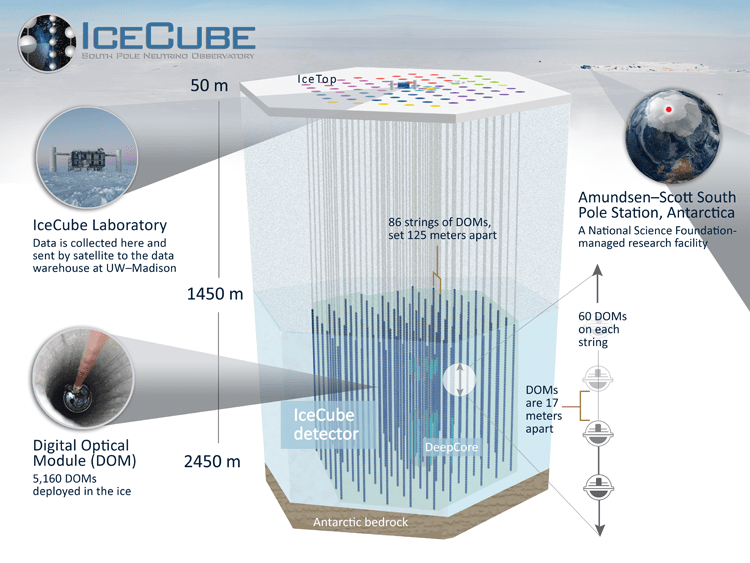
\includegraphics[width=1\linewidth]{figures/icecube.png}
    \caption{Schematic of the IceCube detector. 86 strings carrying a total of 5160 Digital Optical Modules instrument roughly one cubic kilometre of Antarctic ice between 1450\,m and 2450\,m below the surface, with the denser DeepCore sub-array at the bottom centre and the IceTop surface array on top. Figure from the IceCube collaboration \cite{IceCubeWebsite}.}
    \label{fig:icecube}
\end{figure}

The DOMs form the fundamental detection units of IceCube. Each DOM consists of a photomultiplier tube (PMT) and associated electronics enclosed within a pressure-resistant glass sphere. Their purpose is to detect faint flashes of Cherenkov radiation produced by charged particles travelling through the Antarctic ice.

\section{Cherenkov light and DOM readout}
Cherenkov radiation is the optical analogue of a sonic boom. As a charged particle travels through a medium it continuously emits electromagnetic wavefronts, and its motion compresses these waves in the forward direction (Figure~\ref{fig:cherenkov}). If the particle moves faster than the phase velocity of light in the medium, the wavefronts overlap and form a coherent cone of blue light known as Cherenkov radiation. This cone of Cherenkov photons is what the DOMs in IceCube detect~\cite{MartinShaw2019}.

\begin{figure}[H]
    \centering
    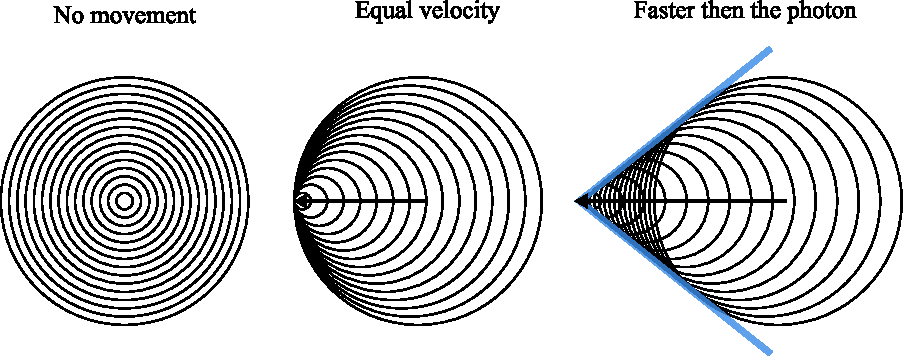
\includegraphics[width=1\linewidth]{figures/shrenkov.pdf}
    \caption{Illustration of Cherenkov radiation. When a charged particle travels through a medium faster than the phase velocity of light in that medium, the emitted wavefronts overlap and form a cone-shaped shockwave of light.}
    \label{fig:cherenkov}
\end{figure}

The charged particles producing this light arise in two main ways. Some are secondary particles, such as muons, electrons, or hadronic showers, created when neutrinos interact with nuclei in or near the detector volume. Others are atmospheric muons, produced in the particle showers that follow when cosmic rays strike nuclei in the atmosphere \cite{IceCube2017}.

When such a particle passes through the detector, the emitted Cherenkov light may reach several nearby DOMs. A DOM that records a signal above threshold registers a hit. A single hit does not by itself define an event. IceCube first asks whether the hit is isolated or whether neighbouring DOMs saw light at nearly the same time~\cite{IceCube2017}.

If a nearest or next-to-nearest neighbouring DOM also records a hit within $\pm 1\,\mu\mathrm{s}$, the hits satisfy the local coincidence condition and are classified as hard local coincidence (HLC) hits. For HLC hits, the digitised signal profile is preserved in the form of ATWD and fADC waveforms, which describe how the detected charge is distributed in time, together with a compact summary \cite{IceCube2017}.

Figure~\ref{fig:hlc_waveform_example} shows an example of the detailed waveform readout stored for a real HLC hit from the 2015 burnsample\footnote{A burnsample is a small subset of real experimental data set aside for testing and validation during analysis development. It is used to study detector and analysis behaviour without exposing the full dataset.}, with the waveforms displayed as calibrated charge per sample in photoelectrons (PE) as a function of time. The upper panel shows the ATWD readout, which samples the prompt part of the pulse every 3.33\,ns and covers a total time window of about 427\,ns. The lower panel shows the fADC readout, which samples every 25\,ns and extends over 6.4\,$\mu$s. The two readouts do not necessarily peak at exactly the same time, as the figure shows, because the ATWD and fADC signals are recorded through different electronics paths with different timing offsets. The ATWD uses a delayed signal path to capture the early part of the pulse, while the fADC samples continuously and stores a longer window after launch \cite{IceCube2017}.

\begin{figure}[H]
    \centering
    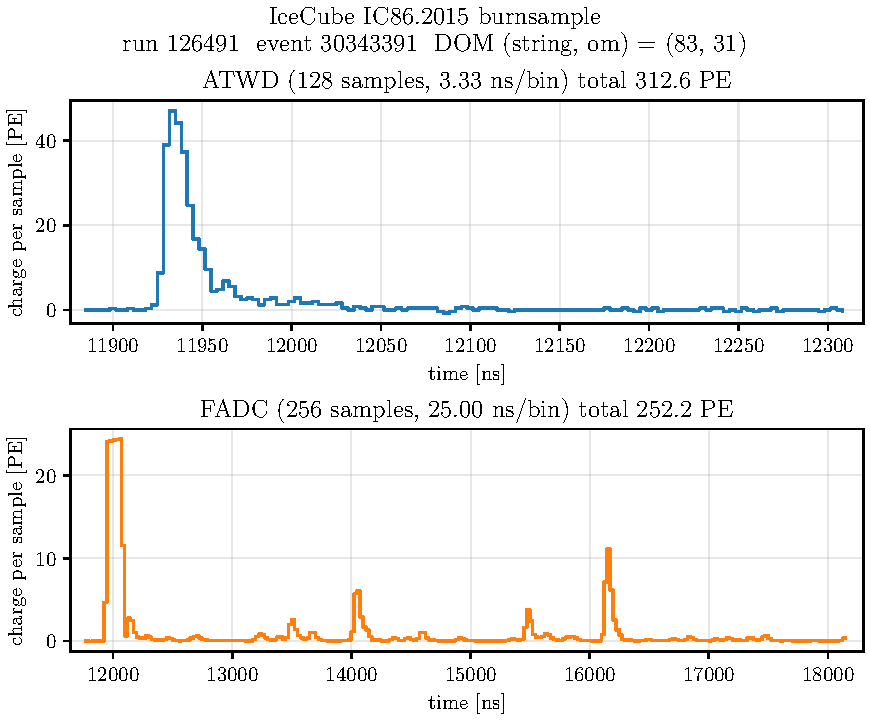
\includegraphics{figures/plot_run126491_event30343391_DOM83-31-0.pdf}
    \caption[Calibrated ATWD and fADC waveforms for a single HLC hit]{
    Calibrated ATWD (top) and fADC (bottom) waveforms for a single
    HLC hit in a DOM in IceCube IC86.2015 burnsample data
    (run 126491, event 30343391, DOM string 83, OM 31). The ATWD covers the
    first 427\,ns at high resolution. The fADC extends to 6.4\,$\mu$s.\protect\footnotemark}
    \label{fig:hlc_waveform_example}
\end{figure}
\footnotetext{This DOM signal is particularly interesting. In the fADC readout, one may notice the small pulses following the main signal. These are not random fluctuations, but afterpulses. They will be discussed later in the analysis.}

In contrast, if no nearest or next-to-nearest neighbouring DOM records a hit within $\pm 1\,\mu\mathrm{s}$, the hit is classified as a soft local coincidence (SLC) hit. For SLC hits, only the compact summary is stored, rather than the full ATWD and fADC waveform readout. This summary includes the hit timestamp, together with a chargestamp consisting of three fADC samples centred around the peak sample and the corresponding peak sample number \cite{IceCube2017}. Table~\ref{tab:hlc_slc_readout_example} shows this compact summary both for the previously mentioned HLC hit and an SLC hit from the same burnsample.

\begin{table}[H]
\centering
\begin{tabular}{rrr}
\toprule
\multicolumn{3}{l}{\textbf{HLC} hit, Run 126491, Event 30343391, DOM (83, 31),} \\
\multicolumn{3}{l}{Hit timestamp $12028.9$ ns, peak index $=7$} \\
\midrule
fADC sample index & $t$ [ns] & PE \\
\midrule
6 & 11922.2 & 4.68  \\
7 & 11947.2 & 24.11 \\
8 & 11972.2 & 24.18 \\
\midrule
\multicolumn{3}{l}{\textbf{SLC} hit, Run 126386, Event 43375646, DOM (20, 1),} \\
\multicolumn{3}{l}{Hit timestamp $180533.7$ ns, peak index $=7$} \\
\midrule
fADC sample index & $t$ [ns] & PE \\
\midrule
6 & -- & 1.03 \\
7 & -- & 3.81 \\
8 & -- & 3.31 \\
\bottomrule
\end{tabular}
\caption{Example compact summaries for one HLC hit and one SLC hit from real IceCube data. Each compact summary contains a three-sample fADC chargestamp centred on the peak fADC sample.}
\label{tab:hlc_slc_readout_example}
\end{table}

The compact summary does not itself contain the fADC sample times. For the HLC hit they can be read off the calibrated fADC waveform. For the SLC hit the full waveform is not stored, which is why the sample times are absent.

These HLC and SLC examples are the closest we come in this report to seeing what an individual DOM actually recorded. The plotted values have been calibrated to PE, but the underlying structure still comes from the raw DOM readout. This raw DOM-level data format is called \texttt{InIceRawData}.

\section{Pulse-level data}
IceCube data do not only exist in this raw form. In the data considered in this report, the DOM readout has already been converted into a simpler pulse-level format called \texttt{SplitInIcePulses}~\cite{WaveDeformDocs}. Instead of keeping raw waveform or chargestamp samples, each DOM hit is represented by one or more reconstructed pulses. Each pulse is described by a small set of values, namely a reconstructed charge, a time label, and the DOM position written as $(x,y,z)$ coordinates. The data also retain information about the DOM itself and whether the hit was classified as HLC or SLC.

We refer to this processed representation as pulse-level data. Table~\ref{tab:pulse_level_combined} shows one complete row from the \texttt{SplitInIcePulses} format, using a real SLC pulse from the 2021 burnsample as an example. It lists both the reconstructed pulse quantities and the associated detector, event, and DOM information, with a short explanation of each variable.
\begin{table}[H]
\centering
\small
\renewcommand{\arraystretch}{1.03}
\setlength{\tabcolsep}{4pt}
\begin{tabular}{@{}lrp{0.58\textwidth}@{}}
\multicolumn{3}{@{}l}{\textbf{Real data event from burnsample 2021}} \\
\toprule
\multicolumn{3}{@{}l}{RunID 135251, EventID 1780, DOM (1,23), pulsemap \texttt{SplitInIcePulses}} \\
\midrule
Variable & Value & Explanation \\
\midrule
\texttt{charge}
& 1.275\,PE
& Reconstructed pulse charge in photoelectrons (PE). It is a pulse-level charge estimate based on the available calibrated DOM signal, either the waveform for HLC hits or the compact chargestamp for SLC hits \cite{IceCube2017,I3RecoPulseTableIO}. \\
\midrule
\texttt{dom\_time}
& 6530\,ns
& Time of the reconstructed pulse, given in ns \cite{I3RecoPulseTableIO}. \\

\midrule
\texttt{dom\_x} & -256.14\,m &
  \multirow{4}{0.58\textwidth}{%
    DOM position in IceCube detector coordinates, given as $(x,y,z)$ in metres. The coordinate origin is located close to the centre of the instrumented detector volume \cite{IceCube2017}.} \\
\texttt{dom\_y} & -521.08\,m & \\
\texttt{dom\_z} &  121.57\,m & \\
& & \\
\midrule
\texttt{hlc} & 0
& Pulse-type flag, with \texttt{hlc} = 1 for HLC hits and \texttt{hlc} = 0 for SLC hits. \\

\midrule

\texttt{rde}
& 1
& Relative DOM efficiency. In this dataset the values are 1.00 and 1.35, where 1.00 corresponds to a standard-efficiency DOM and 1.35 to a higher-efficiency DeepCore DOM \cite{IceCube2017}. \\

\midrule
\texttt{event\_time}
& 59337.887082
& Event-level time label in MJD. For this event it corresponds to 2021-05-03 21:17:23.884800 UTC. \\
\midrule
\texttt{event\_no}
& 0
& Internal event index used in this dataset. Pulses with the same \texttt{event\_no} belong to the same event. \\
\midrule
\texttt{string} & 1 &
  \multirow{2}{0.58\textwidth}{%
    DOM identification variables. \texttt{string} and \texttt{dom\_number} identify the DOM} \\
\texttt{dom\_number} & 23 & \\


\bottomrule
\end{tabular}
\caption{Example of the pulse-level data format used in this report, shown for one DOM signal in the \texttt{SplitInIcePulses} data format.}
\label{tab:pulse_level_combined}
\end{table}

The table lists only the variables used in the coming analysis. Several additional variables exist in the original pulse-level format but are omitted here because they either carry redundant information or are effectively constant in the samples considered. One of these is \texttt{width}, whose relevant information is retained through the derived \texttt{hlc} flag, since widths of $1\,\mathrm{ns}$ and $8\,\mathrm{ns}$ correspond to HLC and SLC hits, respectively.

Table~\ref{tab:pulse_level_combined} shows only a single pulse recorded by one DOM. A full IceCube event consists of many such rows, and the same DOM can appear more than once if it records several pulses within the same event. Together these rows form the pulse-level description of the full event.

\section{Triggers and particle events}
Which pulses belong to the same event is decided by the IceCube trigger and readout system. IceCube uses several trigger algorithms, summarised in Table~\ref{tab:triggers}, to decide when detector readout should be saved as an event. The most common is the Simple Multiplicity Trigger (SMT), which fires when a required number of HLC hits occur within a short time window. Other triggers add simple geometrical requirements, such as clustering hits within a local detector volume or along neighbouring DOMs on the same string. When a trigger condition is satisfied, the event is built from all reconstructed pulses within the corresponding readout window. If several windows overlap, their union defines the event \cite{IceCube2017}.
\begin{table}[H]
\centering
\resizebox{\textwidth}{!}{%
\begin{tabular}{lcccrr}
\toprule
Trigger & DOM set & $N$ HLC hits & Window ($\mu$s) & Topology & Rate (Hz) \\
\midrule
SMT    & in-ice        & 8 & 5   & ---                                  & 2100 \\
SMT    & DeepCore      & 3 & 2.5 & ---                                  & 250 \\
SMT    & IceTop        & 6 & 5   & ---                                  & 25 \\
Volume & in-ice        & 4 & 1   & cylinder ($r=175$\,m, $h=75$\,m)     & 3700 \\
Volume & IceTop infill & 4 & 0.2 & cylinder ($r=60$\,m, $h=10$\,m)      & 4 \\
String & in-ice        & 5 & 1.5 & 7 adjacent vertical DOMs             & 2200 \\
\bottomrule
\end{tabular}%
}
\caption{Trigger parameters (as of May 2016) and typical trigger rates of each algorithm. Most rates vary seasonally with the atmospheric muon flux. Table and caption text adapted from \cite{IceCube2017}.}
\label{tab:triggers}
\end{table}

Many different types of events occur in IceCube, produced by different particle interactions. These include track-like events from muon tracks, cascade-like events from electromagnetic or hadronic showers, and double-bang events from high-energy tau neutrino interactions \cite{Kowalski2017}.

Figure~\ref{fig:icecube_events} from \cite{Kowalski2017} shows examples of these event types at pulse level. The left panel shows a track-like event, the middle a shower-like event, and the right a simulated double-bang event. Each sphere represents a DOM with at least one reconstructed pulse in the event. The sphere size indicates the reconstructed charge, and the colour shows the relative pulse time, with earlier pulses in red and later pulses in blue.

\begin{figure}[H]
    \centering
    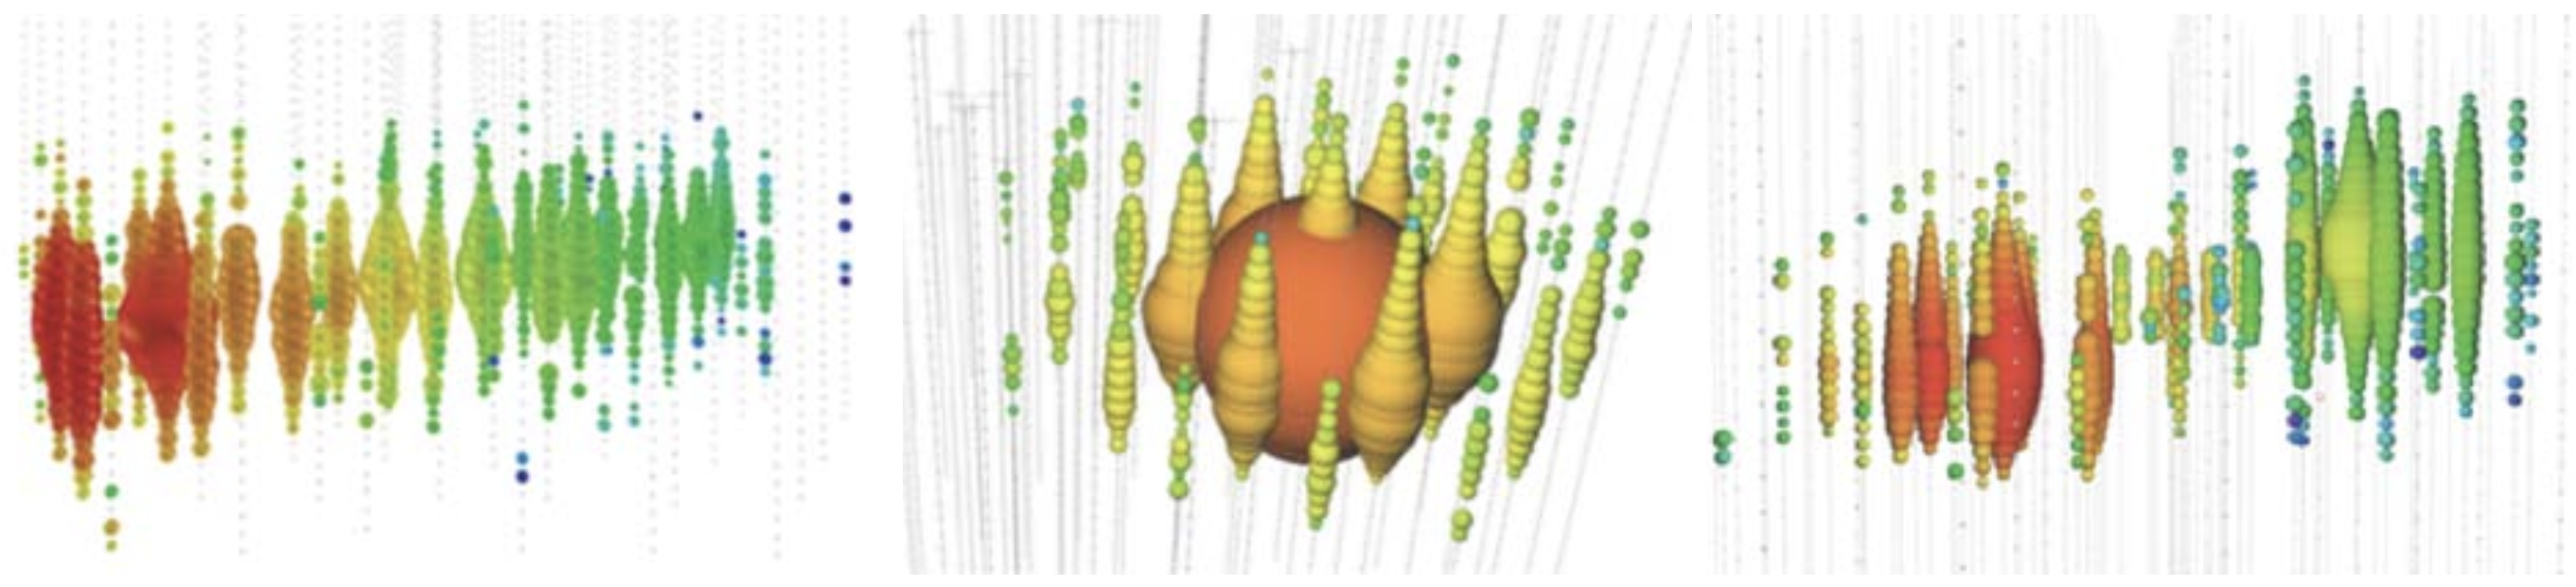
\includegraphics[width=1\linewidth]{figures/icecube_events.png}
    \caption{Examples of IceCube event types shown at pulse level. The track-like (left) and shower-like (middle) events are real detector events, while the double-bang event is simulated. Figure adapted from \cite{Kowalski2017}.}
    \label{fig:icecube_events}
\end{figure}

\section{Real and Monte Carlo data}
As motivated in the introduction, atmospheric muons provide a high-statistics sample of charged-particle tracks in IceCube. The data considered in this report are therefore two samples of atmospheric-muon events, one from real detector data and one from Monte Carlo simulation.

The real-data sample is drawn from the 2021 burnsample and consists of approximately two million events classified as muons using a graph neural network classifier developed by Niels den Besten \cite{DenBestenPrivate}. These events are represented in the \texttt{SplitInIcePulses} pulse-level format.

The corresponding Monte Carlo sample consists of slightly more than two million simulated atmospheric muon events produced with Muon Gun\footnote{Muon Gun is an IceCube tool for efficiently generating single-muon tracks without simulating the full cosmic-ray air shower for each event \cite{VanSanten2020MuonGun}.} and represented in the same \texttt{SplitInIcePulses} format. The Monte Carlo events are produced through a simulation chain of muon propagation through the ice, Cherenkov-photon propagation, detector response, and reconstruction into analysis-level quantities \cite{Meagher2024}, leaving them in the same pulse-level representation as the real data.

These muon events do not all belong to the same physical class. Depending on its energy and trajectory, a muon either crosses the full detector volume or loses enough energy to stop inside it. We call these two cases through-going and stopped muons~\cite{simon}. The two leave distinctly different pulse patterns in the detector (Figure~\ref{fig:event_display_through_stopped} shows one example of each, drawn from our Monte Carlo sample and selected using the truth labels), so treating them as a single homogeneous sample would mix physically distinct event classes when comparing data with simulation.

\begin{figure}[H]
    \centering
    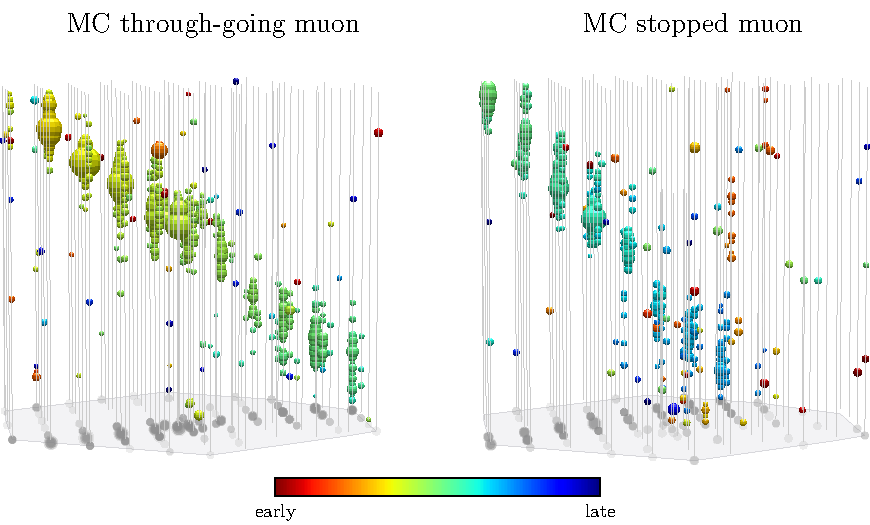
\includegraphics{figures/event_display_through_stopped.pdf}
    \caption{Pulse-level event displays of a through-going (left) and a stopped (right) atmospheric muon from the Monte Carlo sample. Each sphere is a DOM with at least one reconstructed pulse; its size scales with the reconstructed charge and its colour with the relative pulse time, from early (red) to late (blue). The through-going muon produces an extended track that crosses the full instrumented volume, whereas the stopped muon deposits its light along a shorter track that terminates inside the detector.}
    \label{fig:event_display_through_stopped}
\end{figure}

Separating the two classes consistently is where the Monte Carlo truth information becomes essential. Unlike the real data, the simulation carries a truth-level label for every event, and these labels are used to train a supervised classifier that separates through-going from stopped muons. The same classifier is then applied to both Monte Carlo and real data before the comparison is carried out.\footnote{One may ask why the truth labels are not used directly for the Monte Carlo sample. The reason is that no corresponding truth labels exist for real detector data. Applying the same trained classifier to both samples avoids comparing a truth-based split in simulation with a classifier-based split in data.}


\chapter{Machine Learning, the Engine of the Analysis}
That through-going/stopped classifier marks the first time this analysis turns to machine learning, but not the last. This chapter gathers in one place all the machine-learning tools the rest of the report will need. We begin with boosted decision trees and their use in gradient-boosted reweighting, then turn to graph neural networks, and finally to the transformer architecture that does most of the heavy lifting later on.


\section{Boosted Decision Trees}
The treatment of decision trees and boosting in this section is based on Forsyth~\cite{Forsyth2019}.

\subsection{Decision Trees}
A decision tree is a supervised learning model that maps an input vector
\[
    \mathbf{x} = (x_1, x_2, \ldots, x_d)
\]
to a prediction by applying a sequence of binary decisions (Figure~\ref{fig:decision_tree}). Each internal node asks a simple question about one of the input variables. For categorical variables this could be whether the variable belongs to a given category. In this report the relevant input variables are numerical, so the questions are threshold cuts of the form
\[
    x_j < c,
\]
where $x_j$ is one of the input variables and $c$ is a learned threshold.

Depending on the result of the cut, the event is sent to the left or right branch. After a finite number of such decisions it reaches a terminal leaf, where the prediction is made. For classification, the leaf can hold an estimated class probability. For regression or reweighting, it can hold a real-valued prediction.

\begin{figure}[H]
    \centering
    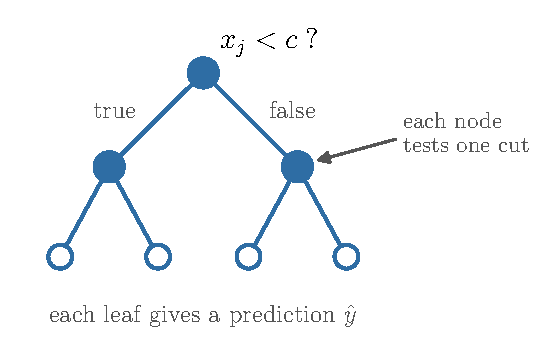
\includegraphics{figures/decision_tree.pdf}
    \caption{A decision tree. Each internal node applies a threshold cut $x_j < c$, and after a sequence of cuts the event reaches a leaf holding the prediction $\hat{y}$.}
    \label{fig:decision_tree}
\end{figure}

A single decision tree is easy to interpret, but usually too simple to capture complicated high-dimensional relations. It may be too shallow to describe the relevant structure, or so deep that it becomes sensitive to statistical fluctuations in the training sample. Boosted decision trees address this by combining many simple trees into one stronger model.

\subsection{Boosting and Gradient Boosting}
That combination is achieved through \emph{boosting}, a sequential training procedure. Instead of fitting one large tree, one fits many shallow trees one after another and adds them together.

Writing the model prediction after $M$ trees as $F_M(\mathbf{x})$, the boosted model is an additive expansion,
\[
    F_M(\mathbf{x})
    =
    \sum_{m=1}^{M} \nu f_m(\mathbf{x}),
\]
where $f_m$ is the $m$-th tree, $M$ the total number of trees, and $\nu$ the learning rate, which controls how much each new tree is allowed to change the current model.

Like almost any machine-learning model, the boosted model is trained by minimising a loss function,
\[
    \mathcal{L}
    =
    \sum_{i=1}^{N}
    L\left(y_i, F(\mathbf{x}_i)\right),
\]
where $y_i$ is the truth for event $i$ and $F(\mathbf{x}_i)$ is the model prediction. The loss measures how bad the current predictions are. For classification, it could penalise wrong class probabilities, and for regression, deviations from a continuous target.

What makes the method \emph{gradient} boosting is how each new tree is chosen. At step $m$, the trees added so far form the current model $F_{m-1}(\mathbf{x})$, and the next tree is fit not to the original target but to the negative gradient of the loss at the current prediction,
\[
    r_i^{(m)}
    =
    -
    \left.
    \frac{\partial L(y_i,F(\mathbf{x}_i))}
         {\partial F(\mathbf{x}_i)}
    \right|_{F=F_{m-1}} ,
\]
the so-called pseudo-residuals, which the next tree approximates,
\[
    f_m(\mathbf{x}_i)
    \approx
    r_i^{(m)}.
\]
Adding that tree to the model is therefore one step of gradient descent, taken in the space of functions rather than over a set of parameters. Figure~\ref{fig:bdt_schematic} summarises the construction.

\begin{figure}[H]
    \centering
    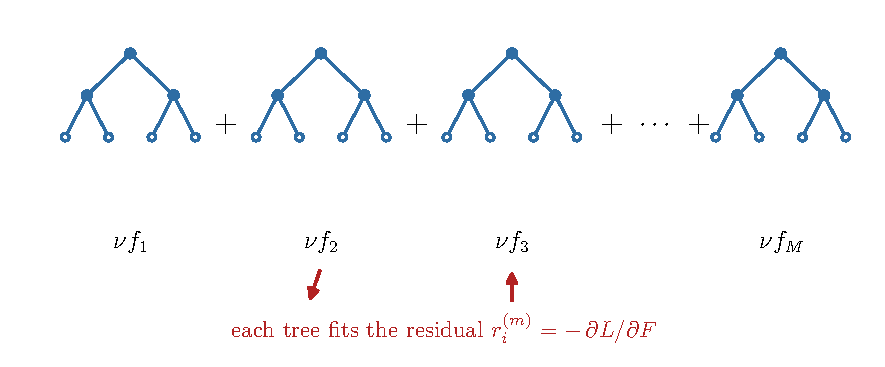
\includegraphics{figures/bdt_schematic.pdf}
    \caption{Illustration of how a boosted decision tree is built up as an additive sequence of shallow trees.}
    \label{fig:bdt_schematic}
\end{figure}

\subsection{Gradient-Boosted Reweighting}
\label{subsec:gb_reweighting}

In this report, boosted decision trees are used through the gradient-boosted reweighter of Rogozhnikov~\cite{Rogozhnikov2016}. The purpose is not to classify events directly, but to assign weights to simulated events so that selected Monte Carlo distributions better match the corresponding distributions in real data.

Ideally, if the data and Monte Carlo samples are described by probability densities
\[
    p_{\mathrm{data}}(\mathbf{x})
    \quad \text{and} \quad
    p_{\mathrm{MC}}(\mathbf{x}),
\]
then the correct event weight would be the density ratio
\[
    w(\mathbf{x})
    =
    \frac{p_{\mathrm{data}}(\mathbf{x})}
         {p_{\mathrm{MC}}(\mathbf{x})}.
\]
Weighting Monte Carlo events by this factor gives larger weights to regions of feature space\footnote{The feature space is the space spanned by the input variables. An event with feature vector $\mathbf{x} = (x_1,x_2,\ldots,x_d)$ corresponds to one point in this space.} where the simulation is underrepresented, and smaller weights where it is overrepresented. The practical difficulty is that the two densities are not known explicitly, especially when $\mathbf{x}$ contains several correlated variables.

Gradient-boosted reweighting avoids estimating the two densities separately by turning the problem into a classification task. A classifier is trained to distinguish data events from Monte Carlo events using the same input variables $\mathbf{x}$. Let
\[
    s(\mathbf{x}) = P(y=1 \mid \mathbf{x})
\]
denote the classifier score, with $y=1$ for data and $y=0$ for Monte Carlo. By Bayes' theorem,
\[
    s(\mathbf{x})
    =
    \frac{\pi_{\mathrm{data}} p_{\mathrm{data}}(\mathbf{x})}
         {\pi_{\mathrm{data}} p_{\mathrm{data}}(\mathbf{x})
         + \pi_{\mathrm{MC}} p_{\mathrm{MC}}(\mathbf{x})},
\]
where $\pi_{\mathrm{data}}$ and $\pi_{\mathrm{MC}}$ are the prior fractions of data and Monte Carlo events in the training sample. Solving for the density ratio gives
\[
    \frac{p_{\mathrm{data}}(\mathbf{x})}
         {p_{\mathrm{MC}}(\mathbf{x})}
    =
    \frac{\pi_{\mathrm{MC}}}{\pi_{\mathrm{data}}}
    \frac{s(\mathbf{x})}{1-s(\mathbf{x})}.
\]
A classifier that separates data from Monte Carlo therefore also contains the information needed to reweight the simulation.

In practice this classifier is a boosted decision tree, and the reweighting is done in a controlled feature space rather than on all available variables at once. Including many variables would in principle let the classifier remove more differences, but it would also make the correction harder to interpret, since the reweighting would no longer isolate which differences are corrected directly and which change only through correlations. The aim is therefore not to force all distributions to be identical, but to apply a controlled correction and then study how it affects the remaining data--Monte Carlo comparison. A boosted decision tree is well suited to this. It gives a flexible but controllable estimate of the density ratio on the few structured tabular variables we allow.


\section{Deep Learning on IceCube Events}

The gradient-boosted reweighter acts on a small set of structured, event-level variables, which is useful when the goal is a controlled correction in a deliberately limited feature space. Many reconstruction and classification tasks in IceCube, however, call for a model that works much closer to the raw detector data, directly on the full, variable-size set of pulses rather than a fixed-length summary, and on the relations between them.

Graph neural networks address this by representing an event as a graph, with the pulses or DOMs as nodes and edges drawn between nodes considered related, for example because they are close in space or time. Each node is then updated by combining its own information with that of its neighbours, so the detector geometry can be built directly into the model through the graph structure. Recent IceCube work applies exactly this idea through the DynEdge architecture and the GraphNeT framework~\cite{DynEdge2022, GraphNeT2023}, where graph neural networks are used for event classification and reconstruction. Through GraphNeT this graph-based approach has become a standard tool in IceCube machine learning. More recently, a growing wave of work has moved beyond fixed graphs toward transformer architectures, and this report follows that wave, replacing the hand-built graph with a transformer that learns which pulses are related from the attention between them.


\section{Transformer Models}
The transformer backbone used here follows Inar Timiryasov's \texttt{iceaggr} architecture~\cite{TimiryasovIceaggr}, while the underlying ideas of self-attention and multi-head attention go back to the original transformer paper of Vaswani et al.~\cite{Vaswani2017Attention}. The description below covers the main components of the architecture at the level of detail used in the rest of this report. In the IceCube setting, the input is one event written as a collection of reconstructed pulses,

\[
    \mathcal{E}
    =
    \left\{
    \mathbf{x}_1,\mathbf{x}_2,\ldots,\mathbf{x}_N
    \right\},
\]
where \(N\) is the number of pulses. Each pulse is described by a feature vector such as
\[
    \mathbf{x}_i
    =
    \left(
    \texttt{charge}_i,
    \texttt{dom\_time}_i,
    \texttt{dom\_x}_i,
    \texttt{dom\_y}_i,
    \texttt{dom\_z}_i,
    \texttt{hlc}_i,
    \texttt{rde}_i
    \right),
\]
drawn from the seven pulse-level quantities of the \texttt{SplitInIcePulses} format introduced in Chapter~\ref{ch:setting_scene}. Which of these a given model actually uses depends on the task, but the key point is that the transformer sees the event as a set of pulses, one feature vector $\mathbf{x}_i$ per pulse.

Before they enter the transformer, each pulse vector $\mathbf{x}_i$ is mapped into a learned latent representation,
\[
    \mathbf{z}_i^{(0)}
    =
    \phi(\mathbf{x}_i),
\]
where \(\phi\) is an embedding network, typically a small neural network or linear projection. This converts the raw pulse variables into a common hidden dimension in which the transformer can process all pulses on equal footing.

The key operation is self-attention. For each pulse representation \(\mathbf{z}_i^{(0)}\), the model constructs three vectors,
\[
    \mathbf{q}_i = W_Q \mathbf{z}_i^{(0)},
    \qquad
    \mathbf{k}_i = W_K \mathbf{z}_i^{(0)},
    \qquad
    \mathbf{v}_i = W_V \mathbf{z}_i^{(0)},
\]
called the query, key, and value, where \(W_Q\), \(W_K\) and \(W_V\) are learned weight matrices shared across all pulses. The query determines how pulse \(i\) measures the relevance of other pulses, the key determines how each pulse is matched against a query, and the value carries the information passed on once the attention weights are computed.

The attention weight from pulse \(i\) to pulse \(j\) follows from the similarity between the query of \(i\) and the key of \(j\),
\[
    a_{ij}
    =
    \frac{
    \exp\left(
    \frac{\mathbf{q}_i \cdot \mathbf{k}_j}{\sqrt{d_k}}
    \right)
    }{
    \sum_{\ell=1}^{N}
    \exp\left(
    \frac{\mathbf{q}_i \cdot \mathbf{k}_{\ell}}{\sqrt{d_k}}
    \right)
    },
\]
where \(d_k\) is the dimension of the key vectors and the factor \(\sqrt{d_k}\) stabilises the scale of the dot products. A large \(a_{ij}\) means pulse \(j\) is considered important when updating pulse \(i\). The attention output for pulse \(i\) is then a weighted sum of the value vectors,
\[
    \widetilde{\mathbf{z}}_i
    =
    \sum_{j=1}^{N}
    a_{ij}\mathbf{v}_j,
\]
so every pulse can receive information from all others, but not equally.

The attention output is then combined with the pulse representation through a residual connection, meaning the layer's input is simply added to its output,
\[
    \mathbf{z}_i^{(1)}
    =
    \mathbf{z}_i^{(0)}
    +
    \widetilde{\mathbf{z}}_i,
\]
so that attention adds information from the rest of the event on top of what each pulse already carried, rather than overwriting it. This sum is then passed through a normalisation layer, which rescales the representations to a stable range so that the values do not grow or shrink uncontrollably as more blocks are stacked.

So far, every pulse has only been updated using information gathered from other pulses. Each pulse representation is now also refined on its own by a feed-forward network, a small network that is applied to one pulse at a time and is identical for every pulse. As with the attention step, its output is added back through a residual connection and passed through a normalisation layer. A single transformer block therefore does two complementary things, namely letting the pulses share information through attention and then refining each pulse representation individually through the feed-forward network.

The attention mechanism described so far is not used just once per block, but several times in parallel, each copy called an attention head. Each head has its own query, key, and value projections and can therefore learn a different notion of relevance. The heads are then combined inside the same block, and stacking several such blocks lets the model build increasingly abstract event representations.

Finally, the pulse representations are reduced to a single event vector. The readout used throughout this report does this with a CLS token, a special extra token added to the list of pulses before the first block. It stands for no real pulse, but takes part in the attention like any other, so by the last of the $L$ blocks its vector, which we write $\mathbf{z}_{\mathrm{CLS}}^{(L)}$, has gathered information from across the whole event and serves as a learned summary of it. This event vector is then passed to a task-dependent prediction head.

Figure~\ref{fig:transformer_architecture} gathers these components into a single overview, from the input pulses to the event-level prediction. With that, the toolbox this chapter set out to assemble is complete, and the transformer is the last and most capable tool in it. Two things are deliberately left open here, the prediction head and the loss the network is trained to minimise. Both depend on what the model is asked to predict and so take a different form from one model to the next, which is why each is introduced only when its model is built in the next chapter.

\begin{figure}[H]
    \centering
    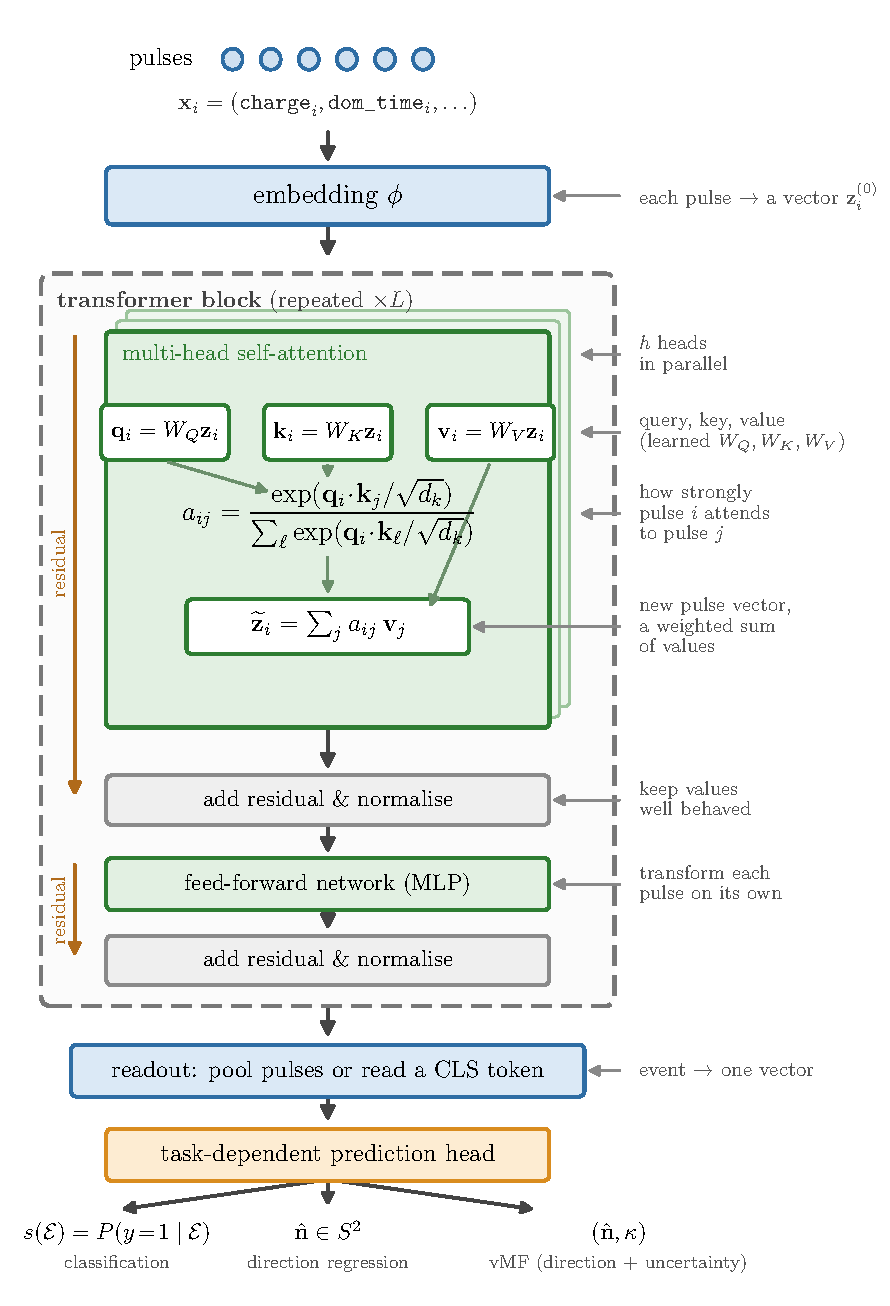
\includegraphics{figures/transformer_architecture.pdf}
    \caption{Simplified overview of the transformer architecture used in this report, from input pulses to the event-level prediction. Each component is described in the text above.}
    \label{fig:transformer_architecture}
\end{figure}


\chapter{Assessing and mitigating discrepancies between real and simulated data}

With the scene now set and the ML engine roaring, we are ready to tackle the central question of this report, how well simulated Monte Carlo data align with real IceCube data, where differences appear, and how they can be mitigated. As mentioned previously, the first step in that process is to separate through-going from stopped muons. Thus, we begin with the through-going/stopped classifier.

\section{The through-going/stopped classifier}
\label{sec:classifier}

The through-going/stopped classifier builds on the transformer backbone of the previous chapter, which we now extend with its own prediction head and loss function. It furthermore carries a set of event-level aggregates, computed deterministically from the pulses, that are fused with the transformer's event representation before the final prediction. The head then reads off a stopped-muon probability, and the network is trained with a cross-entropy weighted to offset the imbalance between the two classes.

\subsection{Event-level aggregates}

The aforementioned event aggregates are ten variables computed directly from the pulses of an event. Labelling the charge, time, and DOM position of the $i$-th pulse as $q_i$, $t_i$, and $\mathbf{r}_i=(x_i,y_i,z_i)$, and writing $N_{\mathrm{pulses}}$ for the number of pulses, the ten variables read

\vspace{-10pt}
\begin{minipage}{0.47\textwidth}
\begin{align}
    N_{\mathrm{pulses}} &= \sum_i 1 \label{eq:nhits}\\
    Q_{\mathrm{tot}} &= \sum_i q_i \label{eq:qtot_cls}\\
    \Delta t &= \max_i t_i - \min_i t_i \label{eq:dt}\\
    \Delta z &= \max_i z_i - \min_i z_i \label{eq:dz}\\
    \sigma_t &= \mathrm{std}\bigl(\{t_i\}\bigr) \label{eq:tstd}
\end{align}
\end{minipage}
\hfill
\begin{minipage}{0.47\textwidth}
\begin{align}
    \mathbf{r}_{\mathrm{mean}} &= \frac{\sum_i q_i\,\mathbf{r}_i}{\sum_i q_i} \label{eq:rcw}\\
    t_{\mathrm{mean}} &= \frac{\sum_i q_i\,t_i}{\sum_i q_i} \label{eq:tcw}\\
    L_{3D} &= \sqrt{(\Delta x)^2 + (\Delta y)^2 + (\Delta z)^2} \label{eq:l3d}
\end{align}
\end{minipage}
\vspace{10pt}

Here $\mathbf{r}_{\mathrm{mean}} = (x_{\mathrm{mean}},y_{\mathrm{mean}},z_{\mathrm{mean}})$ is the charge-weighted centre of light, $t_{\mathrm{mean}}$ its temporal analogue, and $L_{3D}$ the diagonal of the bounding box spanned by the hit DOMs, with $\Delta x$ and $\Delta y$ defined analogously to $\Delta z$. Each of these quantities is physically motivated. A stopped muon deposits its remaining kinetic energy within the instrumented volume and therefore tends to produce a more compact, shorter-lived light pattern, with a centre of light located further from the detector boundaries. A through-going muon instead generates a longer track with a larger spatial and temporal extent. All of this information is, in principle, already accessible to the transformer through its pulse tokens, but providing it explicitly removes the need for the network to reconstruct it from scratch via attention alone.


\subsection{Fusing the aggregates and the training loss}

The transformer summarises each event in its CLS-token vector $\mathbf{z}_{\mathrm{CLS}}^{(L)}$, introduced in the previous chapter. The ten aggregates of the previous section give a second, very different summary of the same event, one we wrote down by hand rather than let the network learn. To use both, the ten aggregates are first passed through a small feed-forward network into an embedding of the same size as the transformer output, and the two vectors are then joined into a single one. This combined vector holds both views of the event at once, the flexible one the network learned for itself and the fixed one we handed it.

This vector is then read off by the prediction head, a small network that turns it into a single number $\ell(\mathcal{E})$, called the logit. A logit can be any real number, so to read it as a probability it is passed through the sigmoid function $$\sigma(\ell(\mathcal{E}))=\frac{1}{1+e^{-\ell(\mathcal{E})}},$$ which maps it into the range from zero to one. This output is the model's estimated probability that the event is a stopped muon. A score near one marks a confident stopped muon and a score near zero a confident through-going one, with the uncertain events left in between.

The network is trained with a binary cross-entropy on the Monte Carlo truth labels, $y=1$ for stopped and $y=0$ for through-going. Through-going events outnumber stopped ones by roughly two to one. Since only the balance between the two classes matters, it is enough to scale the rarer stopped term up by the factor by which it is outnumbered, giving the per-event loss
\[
    L(\ell,y) = -\,\frac{N_{\mathrm{through}}}{N_{\mathrm{stopped}}}\,y\,\log\sigma(\ell) \;-\; (1-y)\,\log\bigl(1-\sigma(\ell)\bigr).
\]


\subsection{Training and performance}

The classifier is trained on the labelled Monte Carlo sample with an 80/10/10 split into training, validation, and test sets. The trained network is then applied without modification to both Monte Carlo and real data, so that the through-going/stopped split is defined consistently in the two samples.

Figure~\ref{fig:cls_training_history} shows the evolution of the training and validation loss together with the validation AUC over the course of training. Training runs in epochs, each a full pass through the training set after which the network has nudged its weights a little closer to fitting the data. A single pass is far from enough, so the set is shown again and again, and after each epoch the network is checked on the held-out validation set to see whether it is still improving or has started to overfit. The validation AUC reaches its best value at epoch 17, marked by the dashed line, and the network from that epoch is the one kept for everything that follows.

\begin{figure}[H]
    \centering
    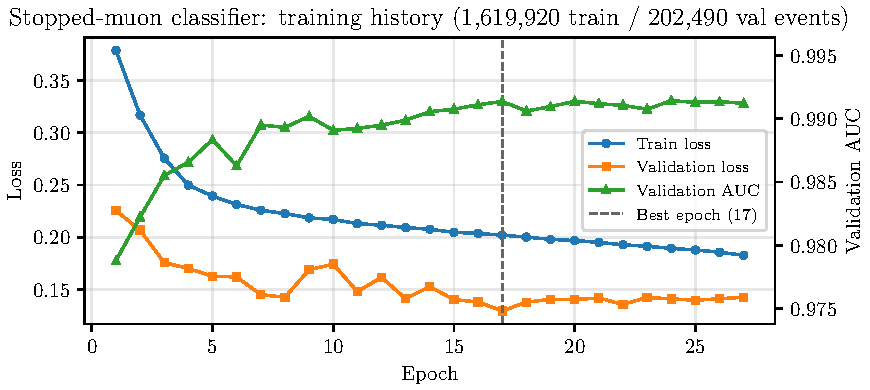
\includegraphics{figures/training_history.pdf}
    \caption{Training history of the through-going/stopped classifier. Training and validation loss is on the left axis, while the validation AUC is on the right axis. The best epoch, used for all subsequent evaluation, is indicated by the dashed line.}
    \label{fig:cls_training_history}
\end{figure}

Figure~\ref{fig:cls_test_performance} summarises the classifier's performance on the held-out Monte Carlo test set. The left panel, the confusion matrix, shows both classes recovered with high accuracy. The right panel is the ROC curve, which traces the true positive rate against the false positive rate as the decision threshold is swept across its range. A perfect classifier would reach the top-left corner, and the curve here sits close to it and well above the diagonal of random guessing, so the model has trained well, rarely raising a false positive while still catching the true events.

\begin{figure}[H]
    \centering
    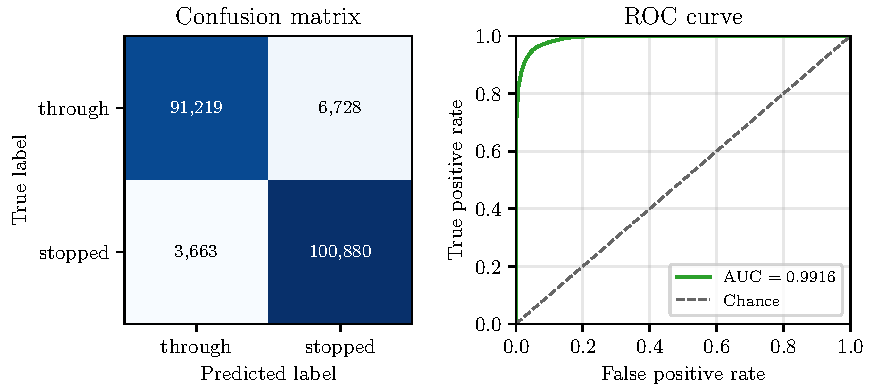
\includegraphics{figures/test_performance.pdf}
    \caption{Test-set performance of the through-going/stopped classifier on MC. The dashed line indicates the chance level.}
    \label{fig:cls_test_performance}
\end{figure}

A complementary view is given in Figure~\ref{fig:cls_score_distribution}, which shows the distribution of the classifier output on the Monte Carlo test set for the two truth classes separately. The left panel displays the logit $\ell$ the prediction head produces, and the right panel the corresponding score $s=\sigma(\ell)$ from the sigmoid.

\begin{figure}[H]
    \centering
    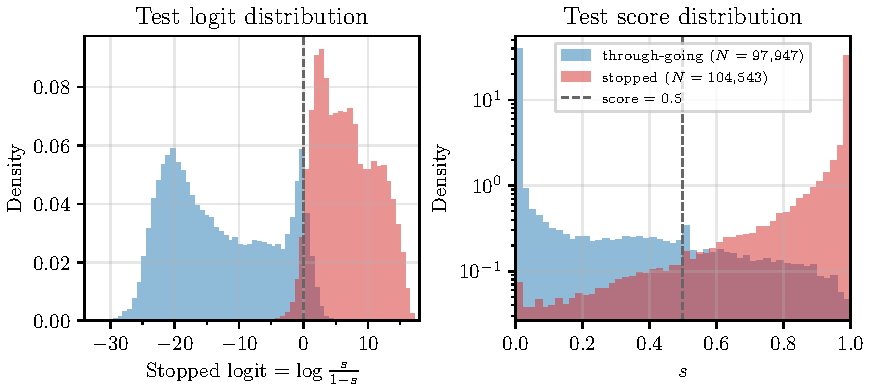
\includegraphics{figures/mc_test_score_distributions.pdf}
    \caption{MC test distributions of the classifier output for the two truth classes.}
    \label{fig:cls_score_distribution}
\end{figure}

In both panels the two classes sit at opposite ends with little overlap, confirming that the model achieved a good separation between through-going and stopped events.

Going forward, several more classifiers will be trained in this report. We will not be repeating the full set of training curves, confusion matrices, and score histograms every time, only when they tell us something worth seeing. Otherwise, we will simply quote the resulting test-set AUC and ask the reader to trust that the same care has gone into the training as above.


\section{Comparing real and simulated data}
\label{sec:data_mc_comparison}

We now apply the trained classifier from the previous section to both the Monte Carlo and the real data, splitting each into through-going and stopped events. With this split in place consistently across the two samples, we can compare simulation and real data on equal footing. A natural first step is to look at the variables that are available in both. We begin at pulse level, where Figures~\ref{fig:pulse_level_variables_page1}--\ref{fig:pulse_level_variables_page2} show the distributions of the pulse-level variables.

\begin{figure}[H]
    \centering
    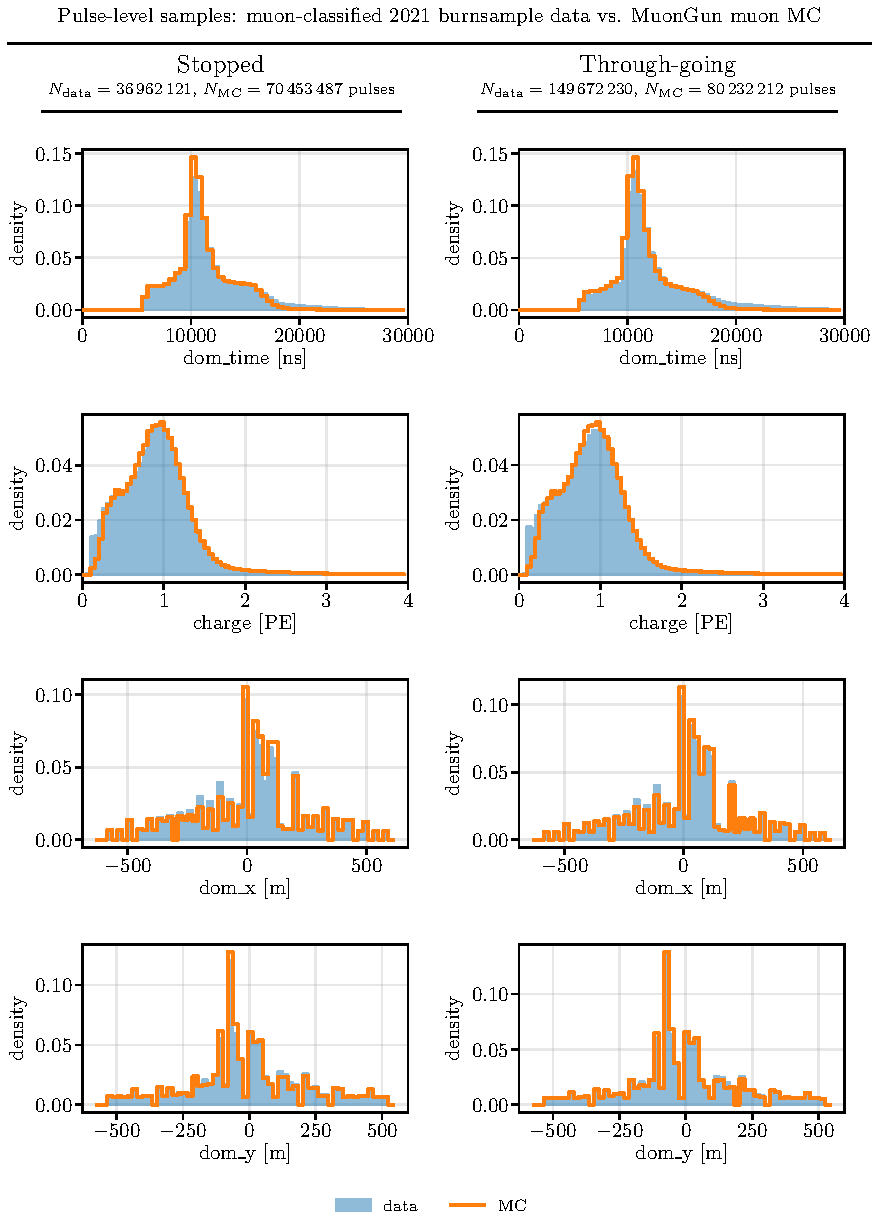
\includegraphics{figures/pulse_level_variables_unmerged_full_page1.pdf}
    \caption{Pulse-level distributions of \texttt{dom\_time}, \texttt{charge}, and the horizontal DOM coordinates \texttt{dom\_x} and \texttt{dom\_y}, shown separately for stopped and through-going events.}
    \label{fig:pulse_level_variables_page1}
\end{figure}

\begin{figure}[H]
    \centering
    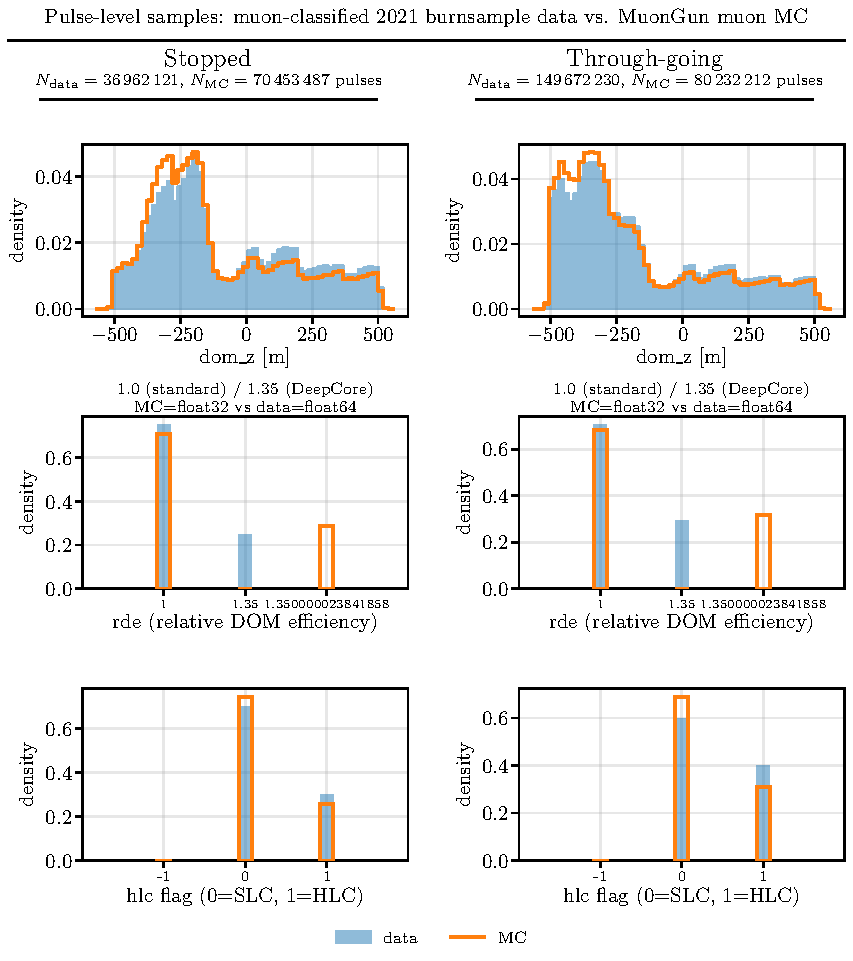
\includegraphics{figures/pulse_level_variables_unmerged_full_page2.pdf}
    \caption{Pulse-level distributions of the vertical DOM coordinate \texttt{dom\_z}, the relative DOM efficiency \texttt{rde}, and the \texttt{hlc} flag, shown separately for stopped and through-going events.}
    \label{fig:pulse_level_variables_page2}
\end{figure}

One technical artefact is immediately visible. The variable \texttt{rde} is stored with slightly different numerical precision in the two samples, in simulation as \texttt{float32} and in real data as \texttt{float64}. This produces small floating-point differences between values that physically represent the same DOM-efficiency category. From a detector point of view the difference is meaningless, but it matters here because we use machine-learning classifiers as a benchmark for how well simulation matches real data. A boosted decision tree or a neural network could trivially exploit the differing numerical representations to separate data from simulation without learning anything physical. The artefact is removed by casting \texttt{rde} to the same floating-point representation in both samples.

Beyond this technical issue, the pulse-level distributions also show several genuine shape differences. Real data contain a small population of low-charge pulses that is not reproduced in MC, and the \texttt{dom\_time} distribution in data has a slightly longer tail toward later pulse times. Smaller disagreements are visible in the horizontal DOM coordinates \texttt{dom\_x} and \texttt{dom\_y}, while the difference is more pronounced in \texttt{dom\_z}. These discrepancies are not removed by a simple technical fix of the input variables. We will return to them after introducing a set of event-level aggregates, since the operation we eventually intend to perform acts on both levels.

These event-level aggregates summarise each event by a small number of quantities derived from its pulses. Several of them have already been defined in the through-going/stopped classifier, and we simply reuse them here. These are the number of pulses $N_{\mathrm{pulses}}$ (eq.~\eqref{eq:nhits}), the total charge $Q_{\mathrm{tot}}$ (eq.~\eqref{eq:qtot_cls}), the time extent $\Delta t = t_{\max} - t_{\min}$ (eq.~\eqref{eq:dt}), the charge-weighted mean time $t_{\mathrm{mean}}$ (eq.~\eqref{eq:tcw}), and the charge-weighted centre of light $\mathbf{r}_{\mathrm{mean}}$ (eq.~\eqref{eq:rcw}), whose vertical component we will denote $z_{\mathrm{mean}}$. To these we add a few new aggregates. For an event with pulses indexed by $i$, pulse charges $q_i$, DOM-times $t_i$, DOM positions $(x_i,y_i,z_i)$, and HLC flags $h_i$, we define

\vspace{-10pt}
\begin{minipage}{0.47\textwidth}
\begin{align}
    N_{\mathrm{DOMs}} &= \left|\{(x_i,y_i,z_i)\}\right|
    \label{eq:n_doms} \\
    Q_{\max} &= \max_i q_i
    \label{eq:qmax} \\
    N_{\mathrm{HLC}}/N_{\mathrm{pulses}} &= \frac{\sum_i h_i}{N_{\mathrm{pulses}}}
    \label{eq:hlc_frac}
\end{align}
\end{minipage}
\hfill
\begin{minipage}{0.47\textwidth}
\begin{align}
    t_{\mathrm{std}} &= \sqrt{\frac{\sum_i q_i (t_i-t_{\mathrm{mean}})^2}{\sum_i q_i}}
    \label{eq:t_q_std} \\
    z_{\mathrm{std}} &= \sqrt{\frac{\sum_i q_i (z_i-z_{\mathrm{mean}})^2}{\sum_i q_i}}
    \label{eq:z_q_std}
\end{align}
\end{minipage}
\vspace{10pt}

The two new count- and charge-like aggregates complement those reused from the classifier. $Q_{\max}$ singles out the largest individual pulse in the event, while $N_{\mathrm{DOMs}}$ counts how many distinct DOMs were hit, regardless of how many pulses each contributed. The HLC fraction $N_{\mathrm{HLC}}/N_{\mathrm{pulses}}$ is the share of HLC-flagged pulses in the event. The two charge-weighted standard deviations $t_{\mathrm{std}}$ and $z_{\mathrm{std}}$ describe how spread out the recorded light is in time and in depth, weighted by pulse charge so that bright pulses contribute more than faint ones. Note that $t_{\mathrm{std}}$ differs from the unweighted time standard deviation $\sigma_t$ used in the classifier (eq.~\eqref{eq:tstd}).

Figures~\ref{fig:event_level_aggregates_page1}--\ref{fig:event_level_aggregates_page3} show the resulting event-level aggregate distributions for stopped and through-going events.

\begin{figure}[H]
    \centering
    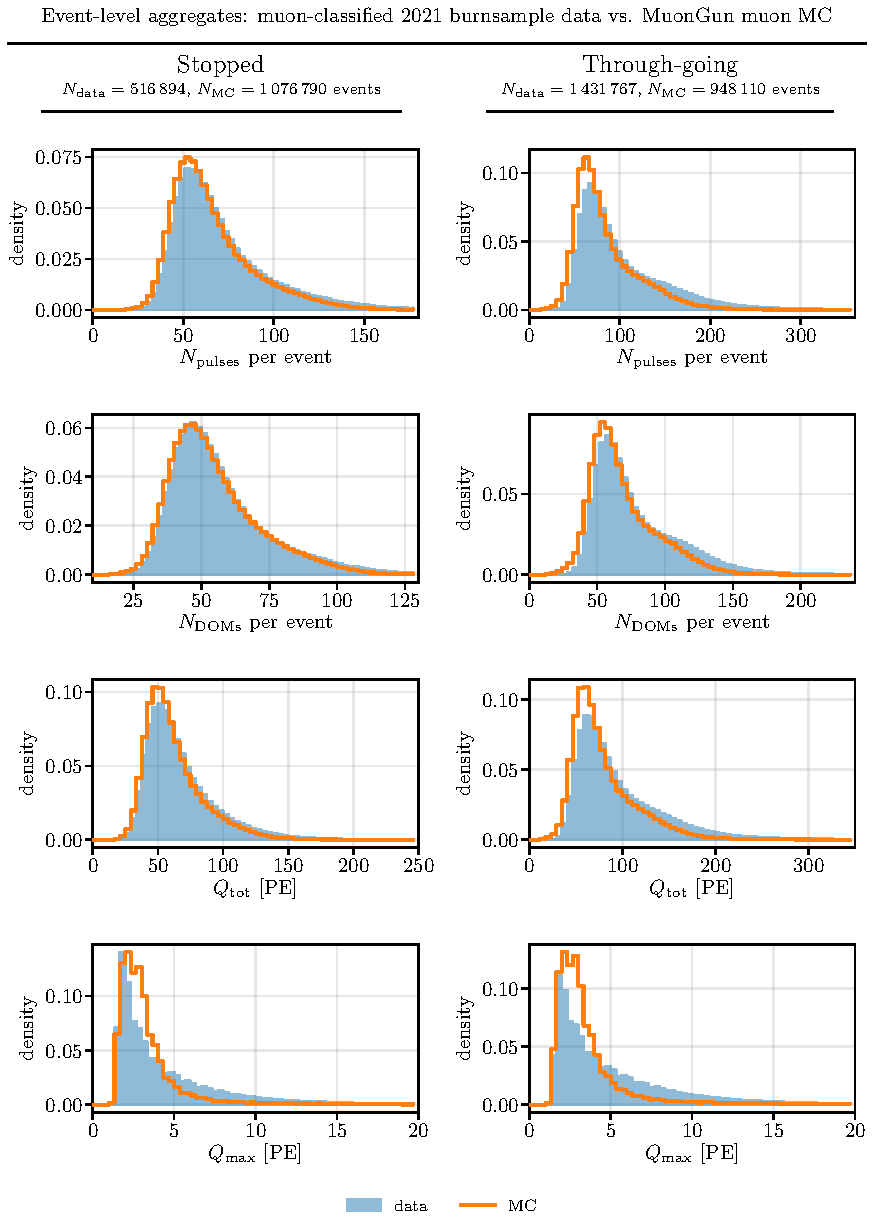
\includegraphics{figures/event_level_aggregates_unmerged_full_page1.pdf}
    \caption{Event-level distributions of the number of pulses $N_{\mathrm{pulses}}$, the number of hit DOMs $N_{\mathrm{DOMs}}$, the total charge $Q_{\mathrm{tot}}$, and the maximum pulse charge $Q_{\max}$, shown separately for stopped and through-going events.}
    \label{fig:event_level_aggregates_page1}
\end{figure}

\begin{figure}[H]
    \centering
    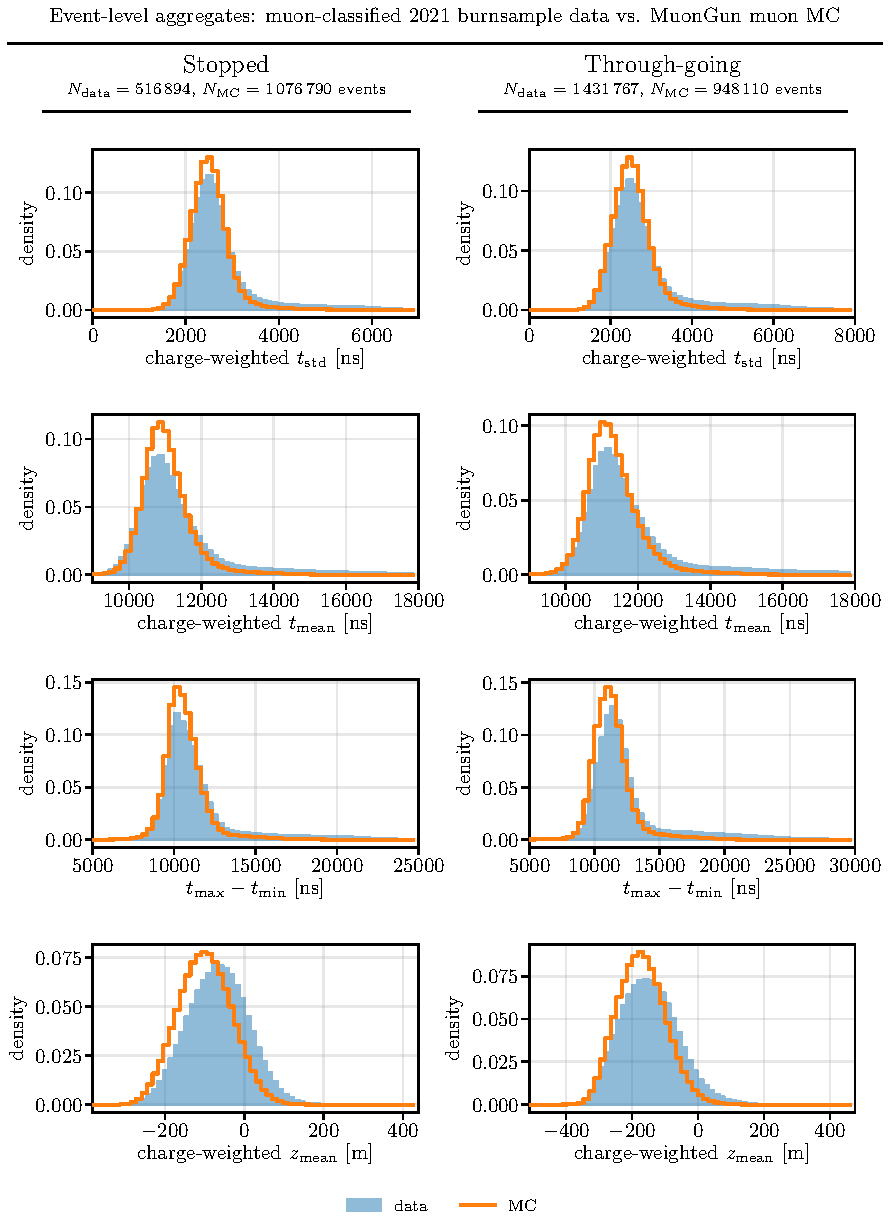
\includegraphics{figures/event_level_aggregates_unmerged_full_page2.pdf}
    \caption{Event-level distributions of the charge-weighted time standard deviation $t_{\mathrm{std}}$, the charge-weighted mean time $t_{\mathrm{mean}}$, the time extent $\Delta t$, and the charge-weighted mean DOM depth $z_{\mathrm{mean}}$, shown separately for stopped and through-going events.}
    \label{fig:event_level_aggregates_page2}
\end{figure}

\begin{figure}[H]
    \centering
    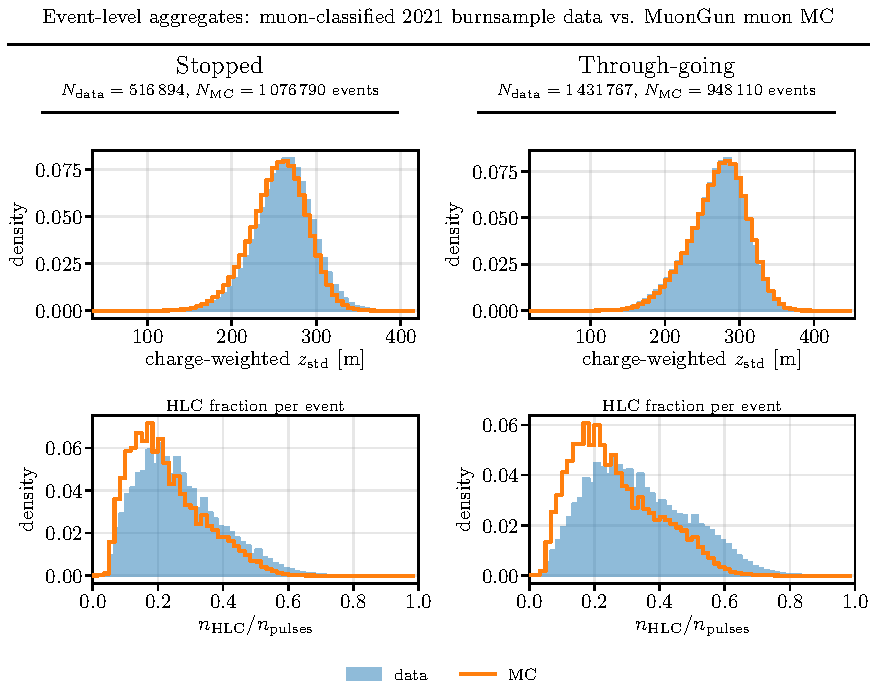
\includegraphics{figures/event_level_aggregates_unmerged_full_page3.pdf}
    \caption{Event-level distributions of the charge-weighted DOM-depth standard deviation $z_{\mathrm{std}}$ and the HLC fraction $N_{\mathrm{HLC}}/N_{\mathrm{pulses}}$, shown separately for stopped and through-going events.}
    \label{fig:event_level_aggregates_page3}
\end{figure}

Several of the pulse-level differences persist after summarising each event. In the first set of aggregates, the data distributions extend further toward large values than MC, most clearly for the through-going sample. This is visible in both $N_{\mathrm{pulses}}$ and $N_{\mathrm{DOMs}}$, where data contain relatively more events with many pulses and many hit DOMs. The same trend appears in $Q_{\mathrm{tot}}$, which is expected since events with more pulses and more hit DOMs generally accumulate more total charge.

The maximum pulse charge $Q_{\max}$ is more interesting because it is not simply a sum over the event. Here data show a noticeably heavier high-charge tail than MC, indicating that individual large-charge pulses occur more often in real data. Beyond this, many of the remaining aggregates tell a similar story. The charge-weighted timing variables and the charge-weighted vertical spread show smaller but consistent differences, with data generally having slightly broader or longer-tailed distributions than MC. The charge-weighted mean depth $z_{\mathrm{mean}}$ shows a more visible shift, consistent with the pulse-level disagreement already seen in \texttt{dom\_z}. The clearest remaining mismatch appears in the HLC fraction, where the data distribution is shifted noticeably toward larger values. Overall, the event-level aggregates confirm the pulse-level observations. Several data--MC differences become more pronounced when the pulses are summarised at event level.

\subsection{A single metric for data--MC distinguishability}
\label{subsec:single_metric}

The histograms above let us see where data and Monte Carlo differ, but they leave a quieter question open. How distinguishable are the two samples when the full set of variables is considered jointly? Each individual disagreement may be modest, yet many small disagreements taken together can amount to a much larger overall mismatch. To compress this question into a single number, we train a classifier to separate data from Monte Carlo using largely the same pulse- and event-level information that has been compared by eye above. The resulting AUC then serves as a benchmark we can keep returning to.

We train the same pulse-level transformer as in Section~\ref{sec:classifier}, with only a handful of changes. The binary label is flipped to $y=1$ for data and $y=0$ for Monte Carlo, and the class weight in the loss is correspondingly the ratio of Monte Carlo to data events in the training set, so the smaller sample is not drowned out. The pulse-level inputs are unchanged, but we instead use all fifteen aggregates, the original ten from eqs.~\eqref{eq:nhits}--\eqref{eq:l3d} together with the five introduced in this section, $N_{\mathrm{DOMs}}$, $Q_{\max}$, $N_{\mathrm{HLC}}/N_{\mathrm{pulses}}$, $t_{\mathrm{std}}$, and $z_{\mathrm{std}}$ (eqs.~\eqref{eq:n_doms}--\eqref{eq:z_q_std}). Including these five is deliberate. They include the ones whose distributions showed the most visible data--MC differences above, and we want the classifier to have access to the discrepancies we are trying to quantify. A separate model is trained for stopped and through-going events, so the diagnostic respects the class splits.

We train each for 20 epochs on an 80/10/10 training/validation/test split of the combined data and Monte Carlo sample.

For stopped events, the classifier reaches a test-set AUC of $0.9882$, and for through-going events $0.9960$. Both sit far above the chance level of $0.5$, and they put a single number on what the histograms in this section have quietly suggested. Real and simulated atmospheric muons are clearly distinguishable.


\section{Reconstructing the event direction}
\label{sec:direction_reco}

The first correction we pursue addresses the incidence direction of the muons. What motivates this is that the shifts in \texttt{dom\_z} and \texttt{dom\_time}, the tail in $N_{\mathrm{pulses}}$ and $N_{\mathrm{DOMs}}$, and the slightly different time extent $\Delta t$ could all result from real and simulated muons entering the detector at different incidence angles. A different angle would mean a different track length through the detector, which would change all of these quantities at once.


To test this, we train a transformer-based reconstruction model on MC to estimate the zenith and azimuth, and apply the same model to both MC and real data. The reconstruction model is built on the same kind of transformer backbone as the through-going/stopped classifier, but with three adjustments.

The first adjustment concerns how the event is presented to the network. Instead of treating each pulse as a token, we treat each DOM as a token, a vector that holds the DOM position together with up to 16 of the pulses recorded on it, zero-padded if there are fewer and truncated to the earliest 16 if there are more.\footnote{Events with more than 256 hit DOMs are likewise truncated to the 256 whose first pulse arrived earliest. In practice this affects only the very largest events.} The second adjustment is that no event-level aggregates are fused in. The last adjustment concerns the output head and the training objective, both of which are adapted to a regression problem on the sphere.

The head is a small feed-forward network that outputs a three-dimensional unit vector,
\[
    \hat{\mathbf{n}} = (\hat{n}_x,\hat{n}_y,\hat{n}_z),
\]
from which the zenith and azimuth are recovered through
\[
    \hat{\theta} = \arccos(\hat{n}_z),
    \qquad
    \hat{\phi} = \mathrm{atan2}(\hat{n}_y,\hat{n}_x) \bmod 2\pi.
\]
The training objective is the opening angle between the predicted and true direction vectors,
\[
    \Delta\Psi(\hat{\mathbf{n}},\mathbf{n}_{\mathrm{true}})
    =
    \arccos(\hat{\mathbf{n}} \cdot \mathbf{n}_{\mathrm{true}}),
\]
averaged over the batch. The model is trained on the Monte Carlo sample using the same 80/10/10 train/validation/test split as the classifier, with the true zenith and azimuth as targets. A single network is trained jointly on stopped and through-going events, so that any class-dependent behaviour seen downstream comes from the events themselves rather than from differences between two separately tuned networks. Training was run for 50 epochs, with the best validation loss at epoch 37. Figure~\ref{fig:dir_opening_angle} unpacks the test-set performance by class. Stopped events have a mean opening angle of $3.96^{\circ}$ and a median of $2.60^{\circ}$, while through-going events are reconstructed somewhat more accurately, with a mean of $3.49^{\circ}$ and a median of $1.92^{\circ}$. The better performance on through-going tracks is consistent with their geometry. A longer track illuminates more DOMs over a larger lever arm, giving the network more information per event from which to constrain the direction.

\begin{figure}[H]
    \centering
    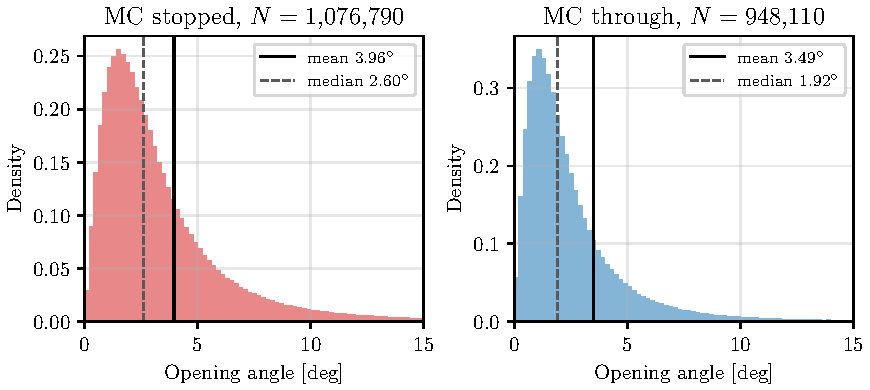
\includegraphics{figures/open_angle_performance.pdf}
    \caption{Per-class opening angle distributions on the held-out Monte Carlo test set.}
    \label{fig:dir_opening_angle}
\end{figure}

With the trained network in hand, the same model is now applied without modification to both Monte Carlo and real data, producing a reconstructed $(\hat{\theta},\hat{\phi})$ for every event in both samples. Figure~\ref{fig:zenaz_overlay} shows the resulting reconstructed zenith and azimuth distributions, with stopped and through-going events for both MC and data overlaid in the same panels.

\begin{figure}[H]
    \centering
    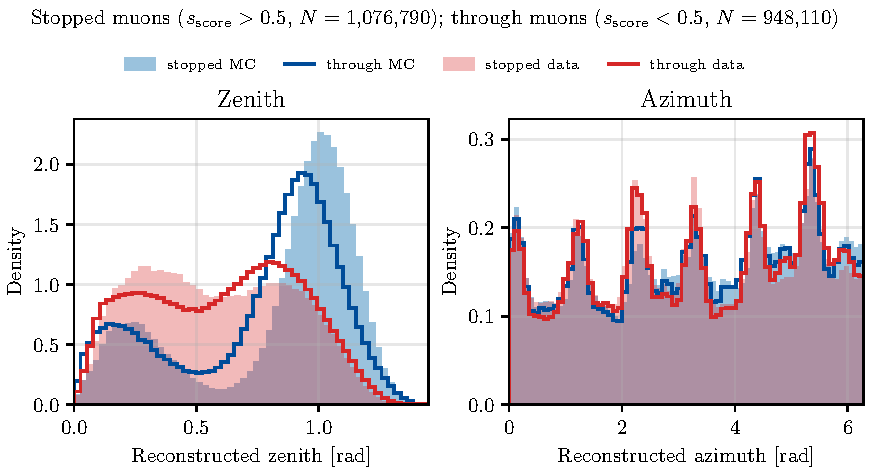
\includegraphics{figures/mc_data_zenith_azimuth_overlay.pdf}
    \caption{Reconstructed zenith (left) and azimuth (right) distributions for stopped- and through-going-classified muons, shown for both MC and 2021 burnsample data.}
    \label{fig:zenaz_overlay}
\end{figure}


The azimuth distributions look much the same in all cases, but the zenith distributions, by contrast, differ markedly. In data the behaviour is as expected. Stopped events sit preferentially at smaller zenith angles and through-going events at larger ones. This makes sense, although two effects compete. An inclined track crosses the detector along a longer chord, which by itself would favour stopping, but a muon that has survived the long slant path to get there tends to be energetic enough to manage the last stretch too. A vertical track instead sees the thinnest possible overburden, so even low-energy muons reach the detector there, and many arrive with only just enough energy to stop inside. The data show the survivor effect winning, with stopped muons clustering toward the vertical. In MC the pattern is reversed, which is a problem in itself, and beyond that the MC zenith distribution differs significantly from data overall.

That data and MC disagree here is of course a problem. Reweighting the simulation on the reconstructed direction $(\hat{\theta},\hat{\phi})$ offers a controlled way to repair it. The angular distributions themselves are pulled into agreement with data, while every other variable can respond only through its genuine correlation with the incoming direction.

\subsection{Applying the angular reweighting}

To do so, we follow Section~\ref{subsec:gb_reweighting} and fit the reweighter with the reconstructed angles as its only input features. It is realised as a boosted decision tree, here configured as a shallow ensemble of 80 trees with maximum depth 3, learning rate $\nu = 0.1$ and at least 200 events per leaf. Separate reweighters are fit for stopped and through-going events, so the correction is allowed to be class-dependent in line with the rest of the analysis. For each Monte Carlo event $i$ the reweighter returns a single multiplicative weight
\[
    w_i^{\mathrm{GB}}
    =
    w_{\mathrm{GB}}\bigl(\hat\theta_i,\,\hat\phi_i\bigr).
\] To avoid the reweighter partially memorising the events it is trained on, the procedure uses two-fold cross-validation. We split the sample into two halves and fit a separate reweighter on each, then weight each half with the reweighter trained on the other. No event is therefore weighted by a model that has seen it during training.

Before looking at how this correction propagates through the rest of the feature space, it is worth checking that it does what it is built to do on its own. As an internal consistency check we train a gradient-boosting classifier (the same model family as the reweighter, with the same hyperparameters) to discriminate data from MC using only $(\hat\theta,\hat\phi)$ as input features, both before and after applying the GB weights. Before reweighting, a small but non-trivial direction-based separation remains, with $\mathrm{AUC}=0.589$ for stopped events and $0.566$ for through-going. After reweighting, both collapse to essentially the chance level, $0.501$ and $0.502$ respectively.\footnote{These values should not be compared directly to the AUCs in Section~\ref{subsec:single_metric}. They are much lower because the classifier here is a small BDT operating on only two input features, $(\hat\theta,\hat\phi)$, whereas Section~\ref{subsec:single_metric} uses the full pulse-level transformer with access to the entire feature space.} The angular information by which data and MC could be told apart in this restricted two-variable space has been almost entirely erased. Figure~\ref{fig:zenaz_gbr} shows the same conclusion graphically. The offset zenith peaks of Figure~\ref{fig:zenaz_overlay}, and the milder azimuth mismatch, now sit on top of one another within each class.

\begin{figure}[H]
    \centering
    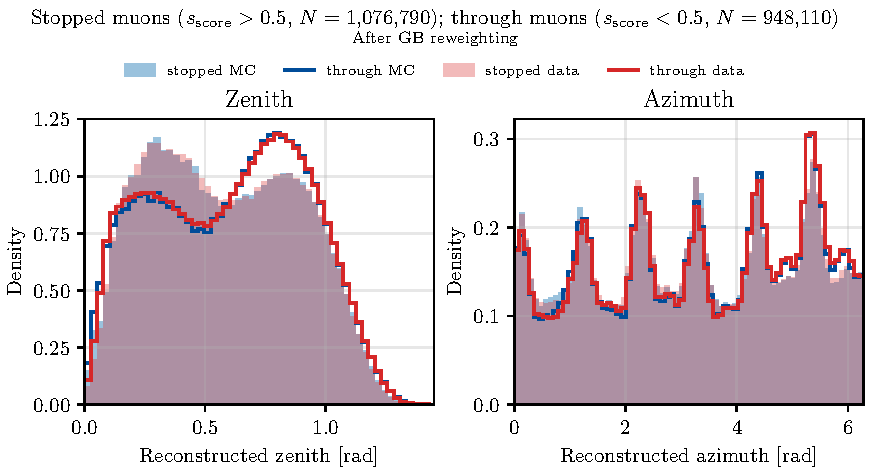
\includegraphics{figures/mc_data_zenith_azimuth_overlay_with_GBR.pdf}
    \caption{Reconstructed zenith (left) and azimuth (right) distributions for stopped- and through-going-classified muons after applying the GB reweighter on $(\hat\theta,\hat\phi)$.}
    \label{fig:zenaz_gbr}
\end{figure}

This sanity check confirms only that the reweighter has succeeded in its own restricted feature space. The more interesting question is what the correction does to every other variable, the ones the reweighter never saw, which are now allowed to respond only indirectly, through their physical and detector-level correlations with the incoming direction. Figures~\ref{fig:pulse_gbr_p1}--\ref{fig:event_gbr_p3} repeat the pulse- and event-level overlays of Section~\ref{sec:data_mc_comparison} with MC drawn both before and after the GB correction.

\begin{figure}[H]
    \centering
    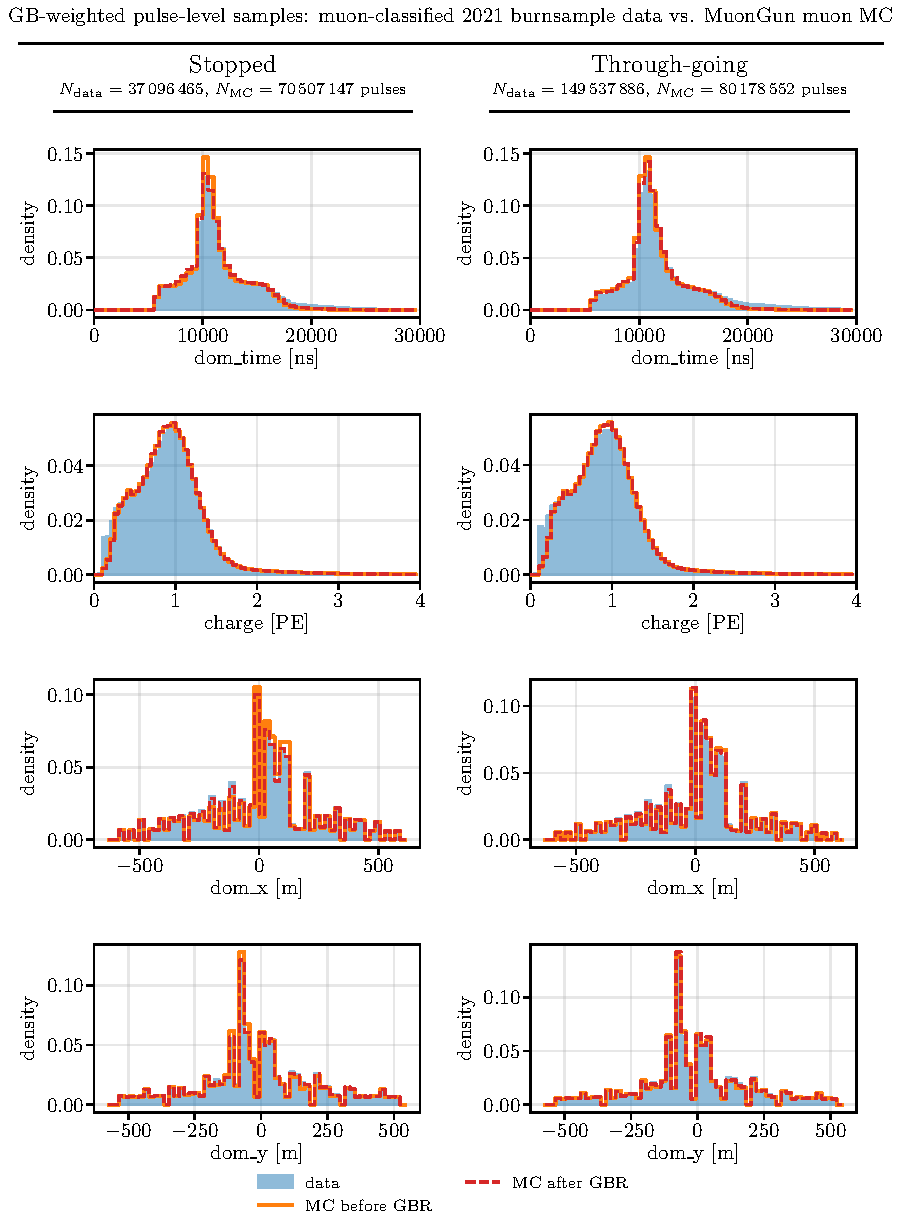
\includegraphics{figures/pulse_level_variables_unmerged_gbweighted_full_page1.pdf}
    \caption{Pulse-level distributions of \texttt{dom\_time}, \texttt{charge}, \texttt{dom\_x}, and \texttt{dom\_y}, with MC shown both before and after the angular GB reweighting. Data is unchanged.}
    \label{fig:pulse_gbr_p1}
\end{figure}

\begin{figure}[H]
    \centering
    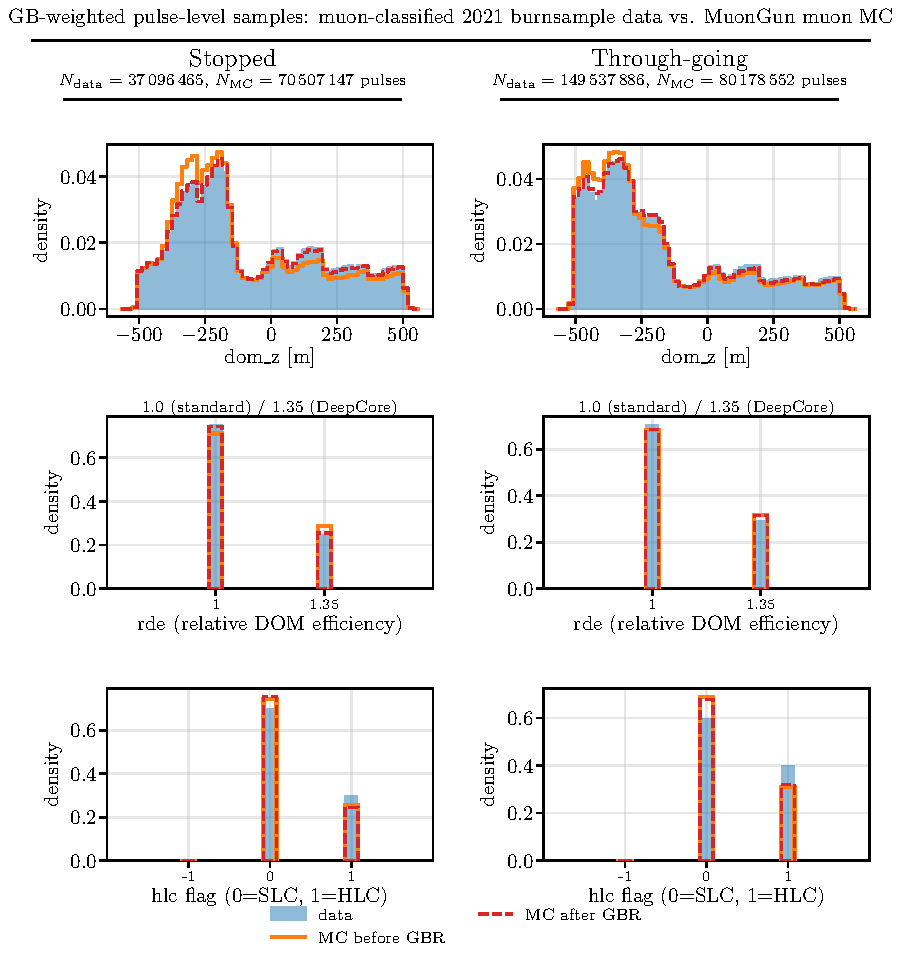
\includegraphics{figures/pulse_level_variables_unmerged_gbweighted_full_page2.pdf}
    \caption{Pulse-level distributions of \texttt{dom\_z}, \texttt{rde}, and \texttt{hlc}, shown before and after the angular GB reweighting.}
    \label{fig:pulse_gbr_p2}
\end{figure}

\begin{figure}[H]
    \centering
    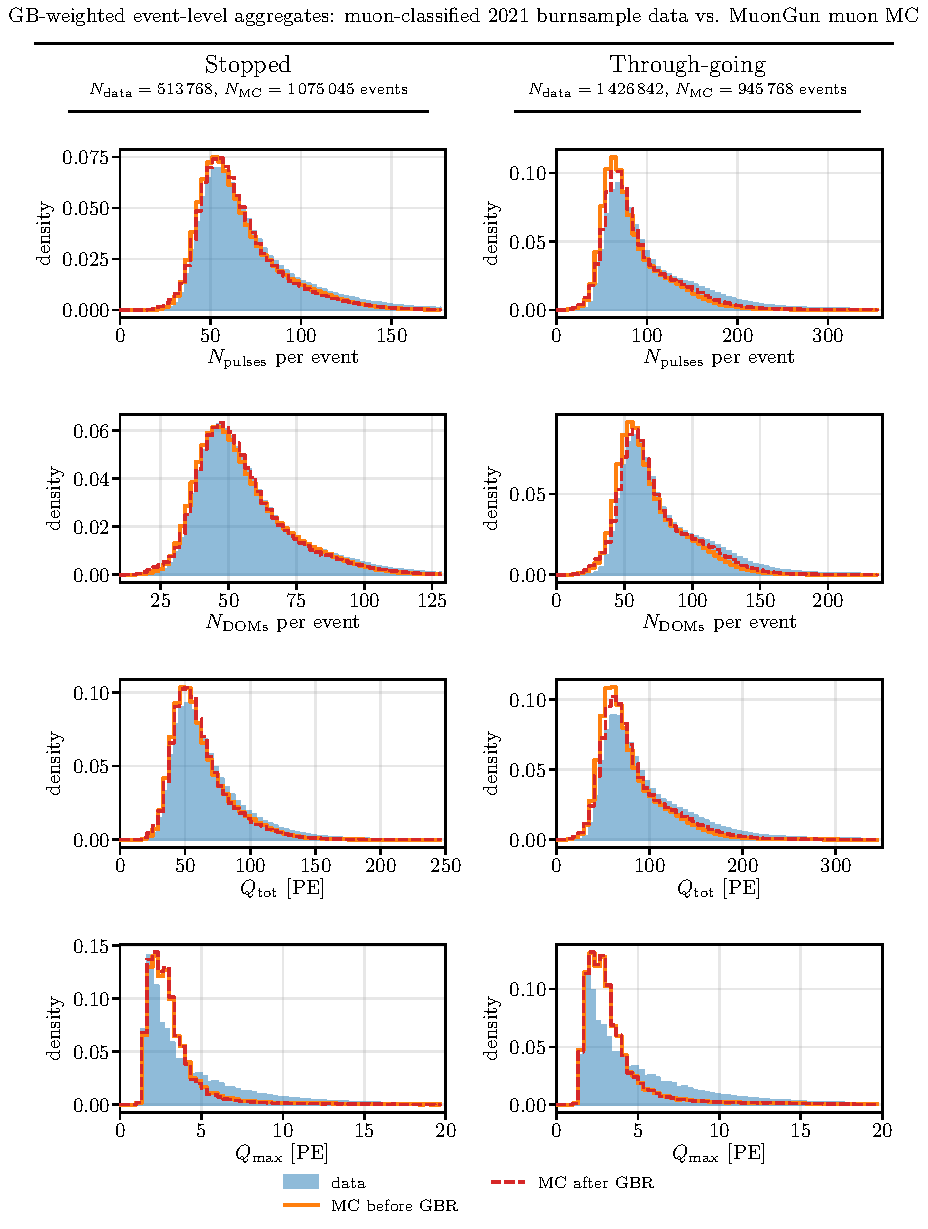
\includegraphics{figures/event_level_aggregates_unmerged_gbweighted_full_page1.pdf}
    \caption{Event-level aggregates $N_{\mathrm{pulses}}$, $N_{\mathrm{DOMs}}$, $Q_{\mathrm{tot}}$, and $Q_{\max}$, shown before and after the angular GB reweighting.}
    \label{fig:event_gbr_p1}
\end{figure}

\begin{figure}[H]
    \centering
    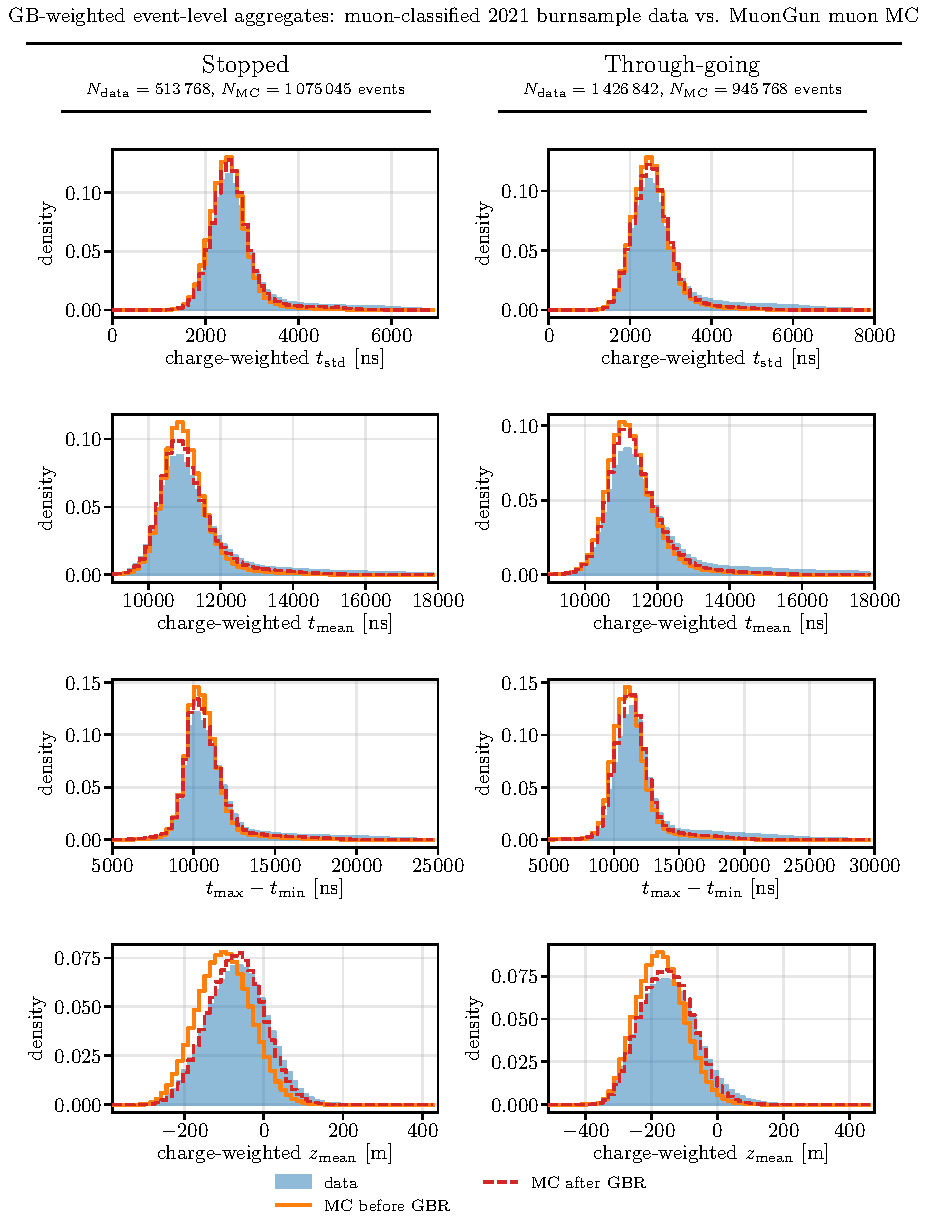
\includegraphics{figures/event_level_aggregates_unmerged_gbweighted_full_page2.pdf}
    \caption{Event-level aggregates $t_{\mathrm{std}}$, $t_{\mathrm{mean}}$, $\Delta t$, and $z_{\mathrm{mean}}$, shown before and after the angular GB reweighting.}
    \label{fig:event_gbr_p2}
\end{figure}

\begin{figure}[H]
    \centering
    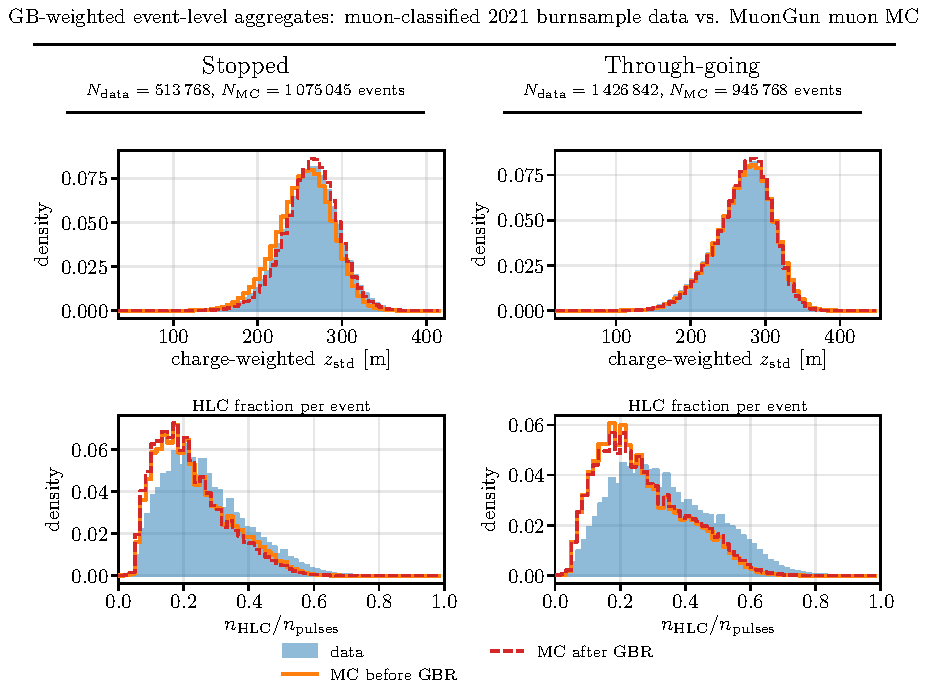
\includegraphics{figures/event_level_aggregates_unmerged_gbweighted_full_page3.pdf}
    \caption{Event-level aggregates $z_{\mathrm{std}}$ and $N_{\mathrm{HLC}}/N_{\mathrm{pulses}}$, shown before and after the angular GB reweighting.}
    \label{fig:event_gbr_p3}
\end{figure}

Across most variables the reweighting produces only a modest improvement in alignment. The exceptions are the depth-related variables \texttt{dom\_z}, $z_{\mathrm{mean}}$, and $z_{\mathrm{std}}$, where the improvement is clearly larger. This is expected, since a shift in zenith translates fairly directly into a shift in the DOM depths visited along the track. The relative DOM efficiency \texttt{rde} improves too, not because it tracks depth itself but because the high-efficiency DeepCore DOMs ($\mathrm{rde}=1.35$) sit in a narrow depth window at the bottom of the detector.

These per-variable observations are encouraging, but the proper question is the one set up in Section~\ref{subsec:single_metric}. We retrain that same MC-vs-data transformer with the same architecture, the same inputs, and the same class split. The only change is that MC events now enter weighted by $w_i^{\mathrm{GB}}$.

The resulting test-set AUC moves from $0.9882$ to $0.9688$ for stopped events, and from $0.9960$ to $0.9935$ for through-going. Both numbers shift in the expected direction, but only slightly, and the classifier still tells data and simulation apart almost perfectly. It is also no accident that the larger improvement belongs to the stopped class. Stopped events had the higher angular AUC to begin with ($0.589$ versus $0.566$), so they had more direction-driven mismatch to remove in the first place. The reconstructed direction is therefore one ingredient of the joint data--MC discrepancy, but only one. Correcting it removes the slice that lives explicitly in $(\hat\theta,\hat\phi)$ and in the depth-like variables strongly correlated with it, but the bulk of the mismatch lies elsewhere, in the remaining pulse- and event-level features that the reweighter never sees.


\section{Pulse merging}
\label{sec:pulse_merging}

As the angular correction has only chipped at the edge of the joint
data--MC mismatch, the remainder must sit in features the reweighter
cannot reach from $(\hat\theta,\hat\phi)$ alone. A natural place to look
is the charge distribution in Figure~\ref{fig:pulse_gbr_p1}, where
the clear low-charge excess in data is left untouched by the angular
correction. A former student and member of the collaboration, S. Debes~\cite{simon}, traced
this excess specifically to the HLC hits and proposed that a fraction
of these sub-$0.3\,\mathrm{PE}$ pulses are not physically independent
but artefacts of the waveform unfolding, where a single physical pulse
is split into a dominant pulse and a smaller satellite~\cite{simon}.

To address this, Debes introduced the \texttt{PulseMerger} algorithm,
which we apply unchanged here. For each DOM, every pulse below a charge
threshold $q_{\mathrm{cut}} = 0.3\,\mathrm{PE}$ is merged into its
nearest above-threshold neighbour in time, with summed charge and
charge-weighted average time,
\[
    q_{\mathrm{merged}} = q_a + q_b,
    \qquad
    t_{\mathrm{merged}} = \frac{q_a t_a + q_b t_b}{q_a + q_b}.
\]
Figure~\ref{fig:pulse_merging_illustration} shows the algorithm at work
on a single DOM from a real 2021 burnsample event. Three
above-threshold pulses (blue) are interleaved with six sub-threshold
pulses (red dashed), each of which is merged into its nearest
above-threshold neighbour in time. The arrows indicate the direction of
the merge. The resulting orange pulses sit close to the original
above-threshold peaks but carry slightly more charge and a marginally
shifted arrival time, reflecting the charge-weighted averaging in the
expressions above.

\begin{figure}[H]
    \centering
    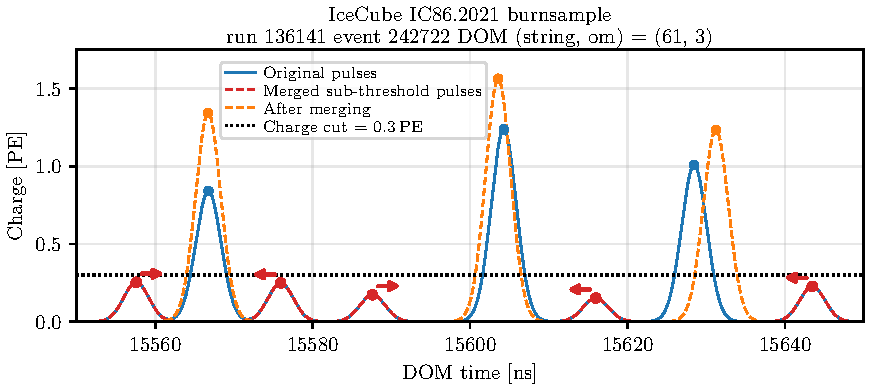
\includegraphics{figures/small_pulses_through_run136141_event242722_string61_dom3_final_legend_default_up.pdf}
    \caption{Illustration of the \texttt{PulseMerger} algorithm on a
    single DOM (string 61, OM 3) from run 136141, event 242722 of the
    IC86.2021 burnsample. Three above-threshold pulses (blue) are
    interleaved with six sub-threshold pulses (red dashed). Each red
    pulse is merged into its nearest above-threshold neighbour in
    time, indicated by the arrows. The resulting merged pulses are
    shown in orange. The dotted line marks the
    $q_{\mathrm{cut}} = 0.3\,\mathrm{PE}$ threshold.}
    \label{fig:pulse_merging_illustration}
\end{figure}

We apply \texttt{PulseMerger} to the full samples.
Figure~\ref{fig:charge_hlc_slc} shows the
per-hit charge distribution split into HLC and SLC hits, with MC and
data overlaid both before and after merging. The HLC panel exhibits
the same low-charge data excess as the one Debes identified \cite{simon}, a clear
bump in data below $0.3\,\mathrm{PE}$ that is absent in MC, producing a
sharp negative dip in the $\mathrm{MC}-\mathrm{Data}$ residual. After
merging, the bump is absorbed into the bulk of the distribution and
the residual flattens. The SLC distribution shows no such low-charge feature to begin
with, and the merging step accordingly leaves it essentially
unchanged.


Having seen that merging cleans up the charge spectrum, it is natural
to ask whether it also helps with a closely related quantity, the
number of pulses recorded per DOM. Figure~\ref{fig:pulses_per_dom}
compares this for HLC and SLC hits, before and after merging. The SLC
distributions already agree, and for HLC hits data carries somewhat
more multi-pulse DOMs than MC, though on the logarithmic scale these
sit in a rare tail and the disagreement is mild. Merging barely moves either comparison. It does pull the HLC per-DOM distributions toward lower multiplicity, since folding away sub-threshold pulses leaves their DOMs with fewer pulses, but it pulls MC and data along together, so their comparison shifts only marginally. The surviving excess sits in the above-threshold multiplicity, which merging never touches.


\begin{figure}[H]
    \centering
    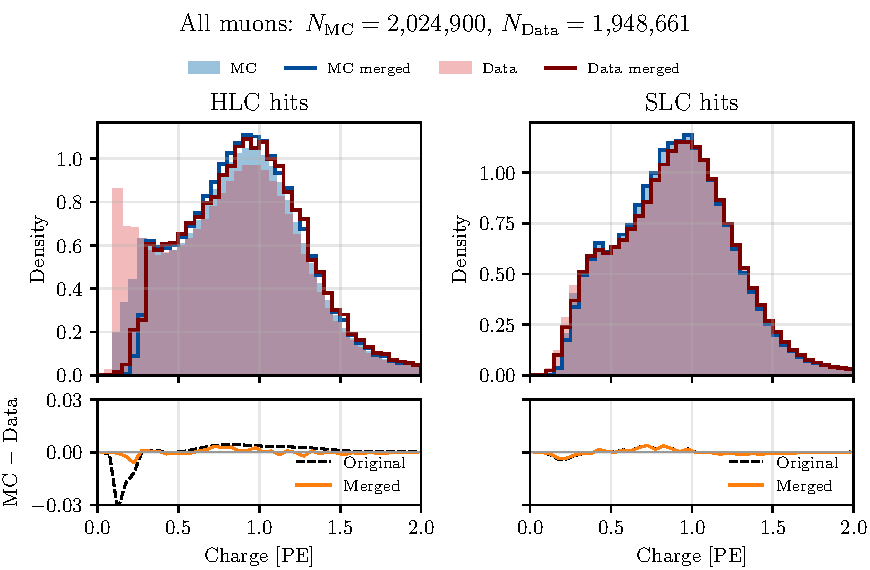
\includegraphics{figures/mc_data_charge_hlc_slc.pdf}
    \caption{Per-hit charge distributions for HLC (left) and SLC
    (right) pulses, shown for MC and data both before and after pulse
    merging. }
    \label{fig:charge_hlc_slc}
\end{figure}


\begin{figure}[H]
    \centering
    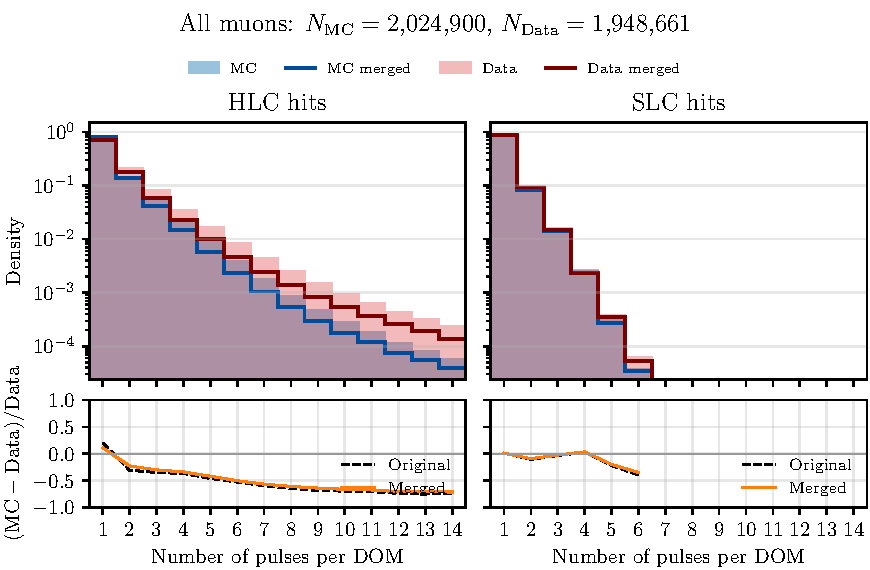
\includegraphics{figures/pulses_per_dom.pdf}
    \caption{Number of pulses recorded per DOM for HLC (left) and SLC
    (right) hits, shown for MC and data before and after pulse merging
    on a logarithmic density scale.}
    \label{fig:pulses_per_dom}
\end{figure}

The global question is again whether this propagates to the AUC of the MC-vs-data transformer. Retraining the same pulse-level transformer as in Section~\ref{subsec:single_metric} on the merged samples gives
$\mathrm{AUC}_{\mathrm{stopped}} = 0.9583$ and
$\mathrm{AUC}_{\mathrm{through}} = 0.9892$. This is a slight improvement from the post-GBR values of $0.9688$ and $0.9935$. The merging removes a
further slice of the mismatch, but, as with the angular reweighting,
only a modest one. The bulk of the data--MC discrepancy survives both
corrections.


\section{Feature importance via permutation}
\label{sec:feature_importance}

The corrections applied so far have each been motivated by a specific physical or technical hypothesis. The angular reweighting targeted a kinematic mismatch first noticed in the reconstructed zenith and azimuth. The pulse merging step targeted a waveform-unfolding artefact identified in earlier work. Each acted on a feature we had a priori reason to suspect, and each removed a real but modest slice of the joint mismatch. We are now in the position of having used up the obvious hypotheses without closing the gap. What remains has to be approached more mechanically. Rather than guessing which feature carries the residual disagreement, we ask the trained classifier itself.

A great tool for this is permutation feature importance. We take the post-merger MC-vs-data transformer from Section~\ref{sec:pulse_merging}, and for each input feature in turn, shuffle its values randomly across all test-set pulses while leaving the others untouched. The resulting drop in AUC,
\[
    \Delta \mathrm{AUC}
    =
    \mathrm{AUC}_{\mathrm{baseline}}
    -
    \mathrm{AUC}_{\mathrm{permuted}},
\]
measures how much the classifier relied on the feature to tell data from simulation, and hence how much of the data--MC mismatch lives in it. We average over several permutations to reduce noise and gauge the stability of the ranking.

Table~\ref{tab:perm_importance_pulse} shows the resulting $\Delta\mathrm{AUC}$ for each pulse-level feature, separately for stopped and through-going events, sorted by the drop observed. The \texttt{hlc} flag leads the ranking by some margin in both classes. This is not a new suspicion, since the HLC fraction $N_{\mathrm{HLC}}/N_{\mathrm{pulses}}$ already stood out in Section~\ref{sec:data_mc_comparison}. The permutation test now makes it the verdict. Among the pulse-level inputs, the HLC/SLC label is the single largest carrier of the residual data--MC distinguishability.

\begin{table}[H]
\centering
\begin{tabular}{lcc}
\toprule
Feature & $\Delta\mathrm{AUC}$ (stopped) & $\Delta\mathrm{AUC}$ (through-going) \\
\midrule
\texttt{hlc}      & 0.296 & 0.428 \\
\texttt{dom\_time} & 0.248 & 0.328 \\
\texttt{dom\_z}    & 0.173 & 0.222 \\
\texttt{dom\_x}    & 0.099 & 0.099 \\
\texttt{dom\_y}    & 0.096 & 0.090 \\
\texttt{charge}    & 0.067 & 0.029 \\
\texttt{rde}       & 0.031 & 0.016 \\
\bottomrule
\end{tabular}
\caption{Permutation feature importance of the pulse-level inputs in the post-merger MC-vs-data transformer.}
\label{tab:perm_importance_pulse}
\end{table}



This points to a natural next step. If the disagreement is concentrated in how the HLC/SLC label is distributed across the pulses, then the simulation is not assigning that label in the same way the real detector does. We cannot rebuild the local-coincidence logic of IceCube from the outside, but we can let a model approximate it for us. We train a classifier on real data to predict whether a given pulse is HLC or SLC from its remaining pulse-level properties, and then apply that classifier to the simulated pulses to re-label them according to the same learned rule. Whether this is enough to move the joint AUC further down is the question of the next section.

\section{Re-labelling HLC pulses}
\label{sec:hlc_flip}

Carrying out that plan first requires a way to measure how close two
HLC-fraction distributions are, since this is the quantity each choice
of flip rate is tuned against. We measure it through the area between
the two empirical CDFs, a quantity known as the 1-Wasserstein distance.
For two histograms $p$ and $q$ that share a binning of width $\Delta x$
with centres $x_k$, it is
\[
    W_1(p,q)
    =
    \sum_{k} \bigl| F_p(x_k) - F_q(x_k) \bigr| \, \Delta x ,
\]
with $F_p$ and $F_q$ the empirical CDFs of $p$ and $q$. Acting on the
CDFs rather than the bins themselves, $W_1$ tracks how far probability
mass is displaced between the two distributions, not just whether the
bins differ.

\subsection{A data-trained HLC classifier}

The classifier we use is the pulse-level transformer of
Section~\ref{sec:data_mc_comparison} with three changes. The
\texttt{hlc} flag is moved from input to target, the head is per-pulse
instead of per-event, and no event-level aggregates are fused in. The remaining
pulse-level inputs are unchanged.

With this, we train the transformer model on the real data and for comparison we also train a DynEdge GNN with the same feature inputs, included purely as a cross-check on the
transformer's ranking. Both reach near-perfect test-set performance,
\[
    \mathrm{AUC}_{\mathrm{Transformer}}
    =
    \bigl(0.9997,\ 0.9998\bigr),
    \qquad
    \mathrm{AUC}_{\mathrm{DynEdge}}
    =
    \bigl(0.9993,\ 0.9995\bigr),
\]
for (stopped, through-going).

\subsection{Flipping the most HLC-like SLC pulses}

With that classifier in hand, we now apply it to the simulation. Every
SLC pulse in the MC sample is scored by how HLC-like the data-trained
model finds it, and the pulses are then ranked by this score. The top
$x\%$ have their \texttt{hlc} flag flipped from $0$ to $1$, while the rest are left untouched.

The flip rate $x$ is set by minimising the $W_1$ distance between the
MC and data $N_{\mathrm{HLC}}/N_{\mathrm{pulses}}$ distributions.
Figure~\ref{fig:hlc_flip_sweep} shows the resulting sweep, separately
for stopped and through-going events and for the two models.

\begin{figure}[H]
    \centering
    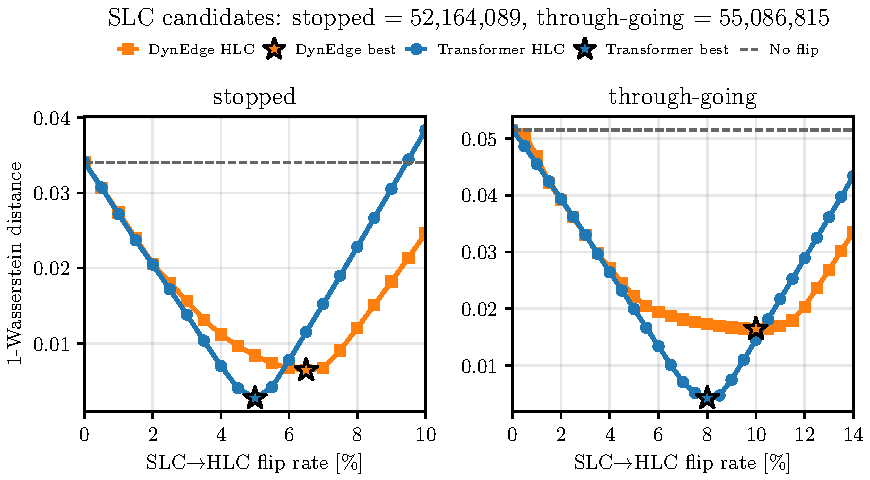
\includegraphics{figures/hlc_flip_rate_sweep_merged_v2_stopped_through_side_by_side_0_to_10p0_step0p5.pdf}
    \caption{1-Wasserstein distance between the MC and data $N_{\mathrm{HLC}}/N_{\mathrm{pulses}}$ distributions as a function of the SLC$\to$HLC flip rate, for stopped (left) and through-going (right) events. Stars mark each model's optimum. The dashed line is the no-flip baseline.}
    \label{fig:hlc_flip_sweep}
\end{figure}

The transformer reaches a lower minimum than DynEdge in both classes and does so at a
smaller flip rate, concentrating the re-labelling in fewer pulses. We
adopt the transformer at its per-class optimum.
Figure~\ref{fig:hlc_frac_flipped} shows the resulting HLC-fraction
distributions after applying the flip. The MC, which sat clearly to the left of
data before the flip, now tracks data closely across the full range.

\begin{figure}[H]
    \centering
    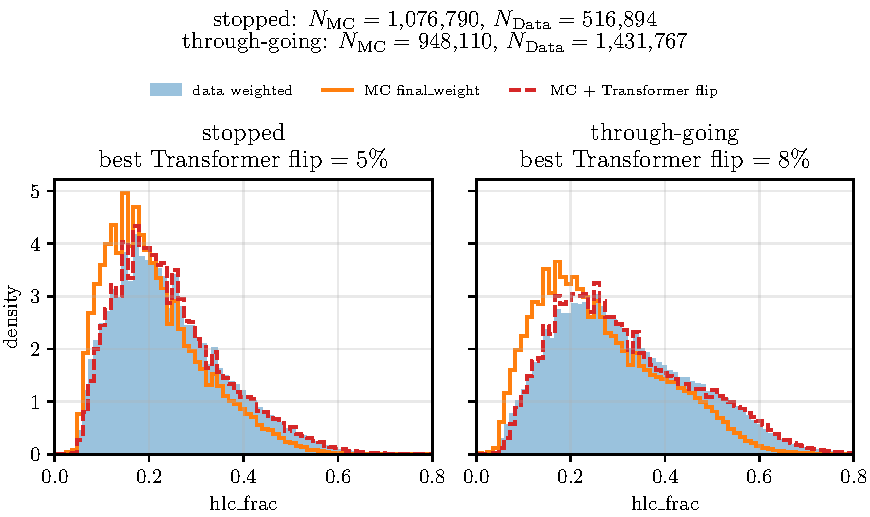
\includegraphics{figures/hlc_frac_mc_vs_data_merged_v2_stopped_through_best_transformer_flip_side_by_side.pdf}
    \caption{HLC-fraction distributions for stopped (left) and through-going (right) events, comparing data (blue), the reweighted and merged MC (orange), and the same MC after the best-transformer SLC$\to$HLC flip (red dashed).}
    \label{fig:hlc_frac_flipped}
\end{figure}

A clean match in one variable need not translate into a smaller joint
mismatch, so we retrain the MC-vs-data transformer of
Section~\ref{sec:data_mc_comparison} on the post-flip samples. The
test-set AUC drops to $0.9281$ for stopped, from $0.9583$ after pulse
merging, and to $0.9851$ for through-going, from $0.9892$. For stopped
events this is the largest single-step improvement in this analysis,
confirming that the permutation test pointed at the right feature. The HLC label
is not the only carrier of residual disagreement (the joint
classifier still separates data from simulation clearly), but
it is the most consequential one yet identified.


\section{Charge versus time}
\label{sec:charge_time}


We now turn to a known effect in real data that is not simulated in MC. These are the afterpulses introduced in Chapter~\ref{ch:setting_scene}, which appear as small delayed pulses trailing the main fADC signal in Figure~\ref{fig:hlc_waveform_example}. They are a common feature of PMTs and are attributed to the ionisation of residual gas inside the tube by electrons that are accelerated between the dynodes. The resulting ions drift back and release further electrons, producing secondary pulses up to several microseconds after the primary signal \cite{IceCube2017}. Since they are present in data but absent from MC, they should
leave a data excess in the joint distribution of pulse charge and pulse time. We therefore
look at the \texttt{charge}--\texttt{dom\_time} plane directly, where an
afterpulse population would appear as a delayed, low-charge cloud offset
from the prompt light and stronger in data than in MC.

Figures~\ref{fig:afterpulse_stopped_mc}--\ref{fig:afterpulse_through_res}
show this plane for stopped and through-going events. We observe a similar structure in both samples, although data extends to later times than MC and is generally more spread out.

We do not, however, find the afterpulses. There is no isolated delayed island to point to. One explanation is that afterpulses may not occur very often at the low pulse charges between 0 and 2 PE, where most of our pulses lie. Another explanation is that once the data are converted from the raw waveforms to the pulse-level format, the afterpulse signature is washed out.

\begin{figure}[H]
    \centering
    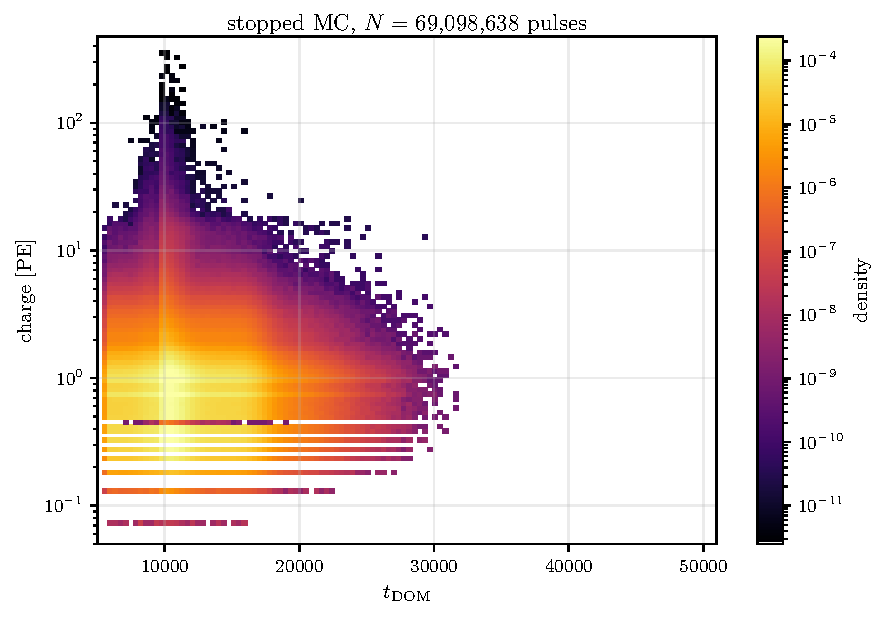
\includegraphics{figures/afterpulse_stopped_mc_transformer_hlcflip_best.pdf}
    \caption{Charge versus pulse time for stopped MC.}
    \label{fig:afterpulse_stopped_mc}
\end{figure}
\begin{figure}[H]
    \centering
    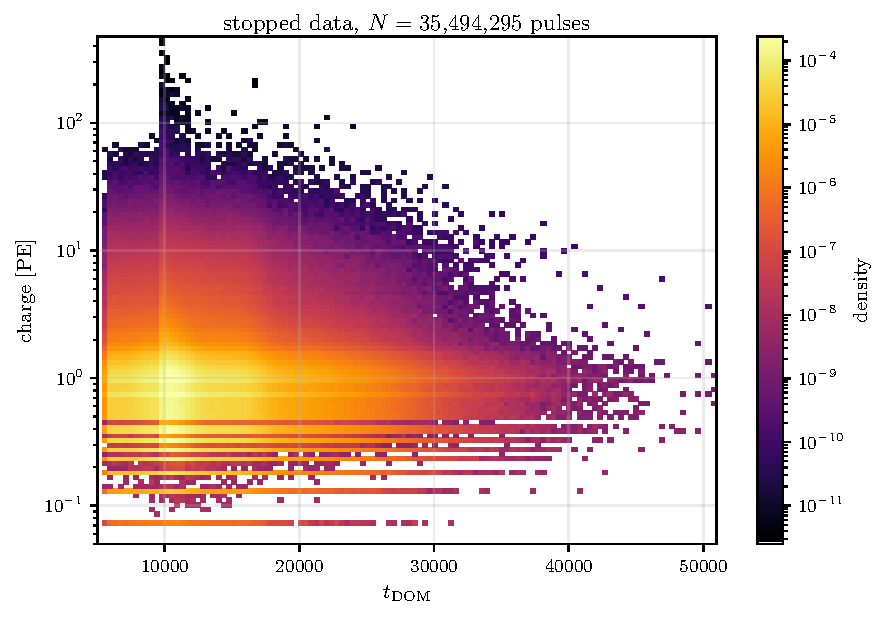
\includegraphics{figures/afterpulse_stopped_data_transformer_hlcflip_best.pdf}
    \caption{Charge versus pulse time for stopped data.}
    \label{fig:afterpulse_stopped_data}
\end{figure}
\begin{figure}[H]
    \centering
    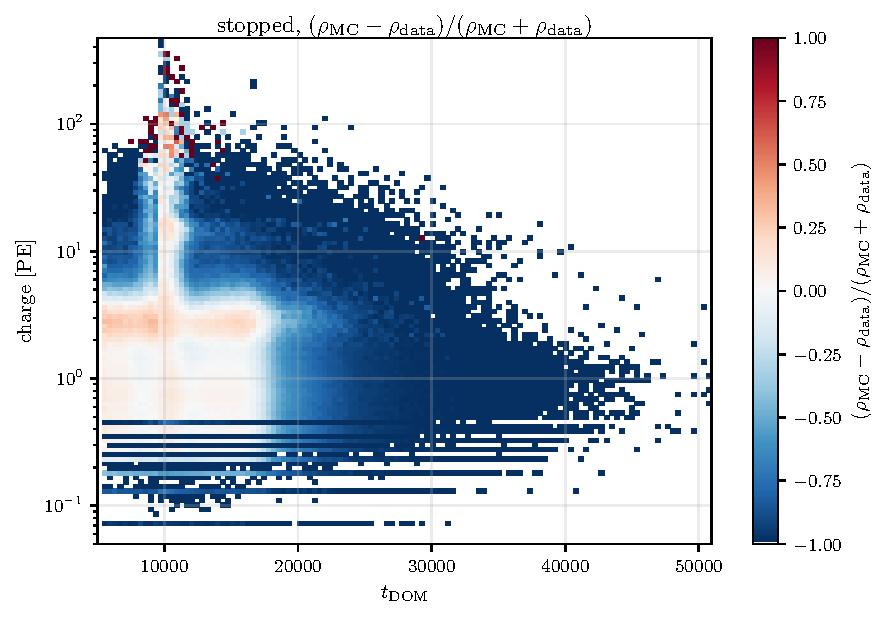
\includegraphics{figures/afterpulse_stopped_mc_over_data_transformer_hlcflip_best.pdf}
\caption{Normalised charge--time residual, stopped events.}
    \label{fig:afterpulse_stopped_res}
\end{figure}
\begin{figure}[H]
    \centering
    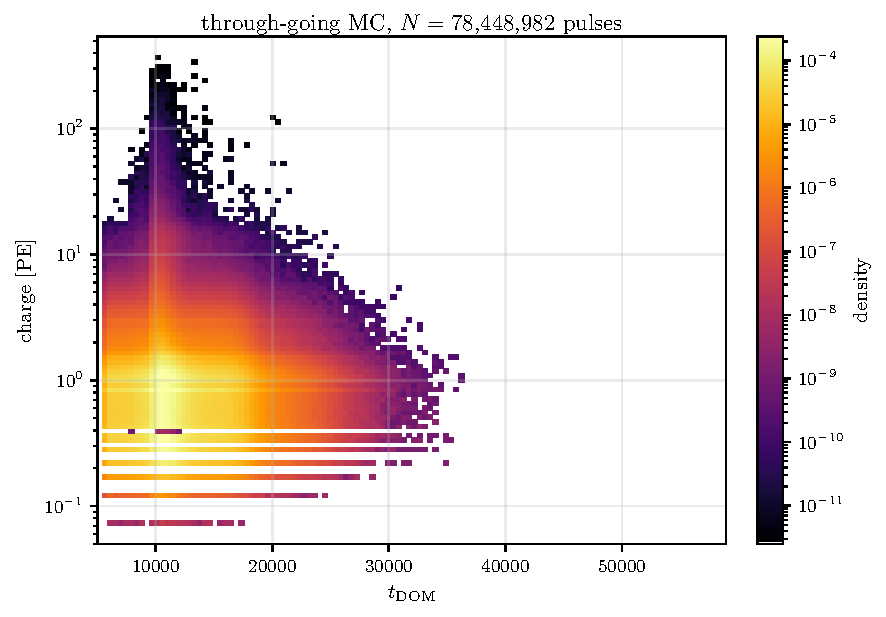
\includegraphics{figures/afterpulse_through_mc_transformer_hlcflip_best.pdf}
    \caption{Charge versus pulse time for through-going MC.}
    \label{fig:afterpulse_through_mc}
\end{figure}
\begin{figure}[H]
    \centering
    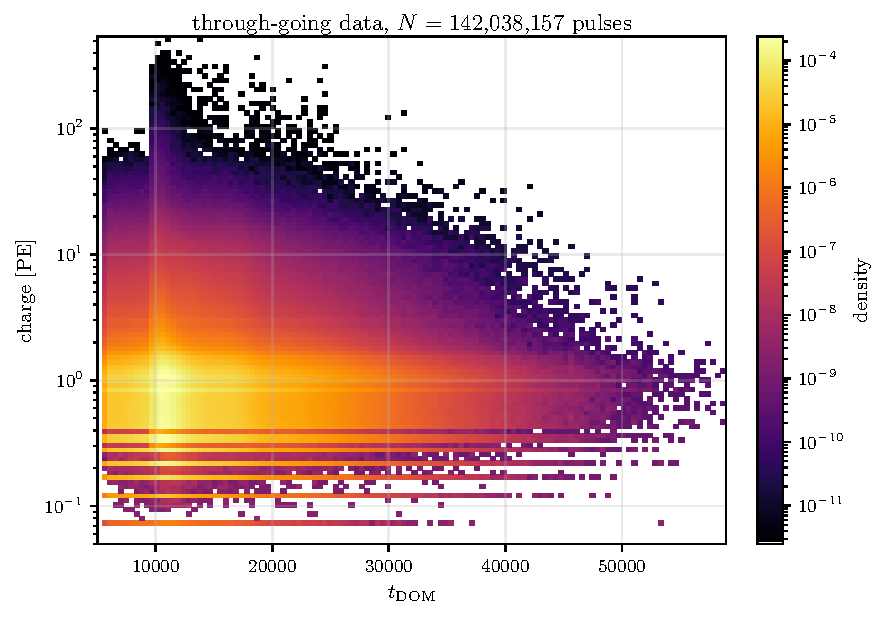
\includegraphics{figures/afterpulse_through_data_transformer_hlcflip_best.pdf}
    \caption{Charge versus pulse time for through-going data.}
    \label{fig:afterpulse_through_data}
\end{figure}
\begin{figure}[H]
    \centering
    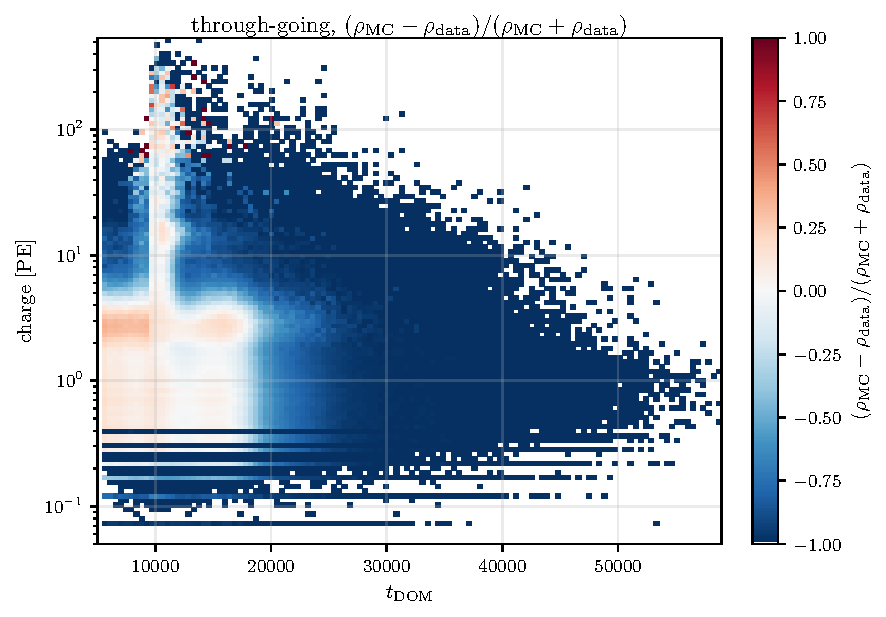
\includegraphics{figures/afterpulse_through_mc_over_data_transformer_hlcflip_best.pdf}
    \caption{Normalised charge--time residual for through-going events.}
    \label{fig:afterpulse_through_res}
\end{figure}

Every comparison up to this point has concerned a property of the events
themselves, whether recorded directly, like the pulses and their HLC labels, or
estimated from them, like the reconstructed angles. We close the analysis with
a comparison of a different nature, on a quantity that describes the
reconstruction rather than the muon, namely how confidently each event can be
placed on the sky.

\section{A learned per-event uncertainty as a final diagnostic}
\label{sec:vmf}

The directional model from Section~\ref{sec:direction_reco} reconstructs a direction $(\hat\theta,\hat\phi)$ for each event. This is a point estimate and nothing more. It says where the muon came from, but not how well that direction is constrained. As a final diagnostic, we therefore let the same model estimate this uncertainty as well, using the von Mises--Fisher (vMF) prediction head adopted from Happel~\cite{happel}.
Instead of a single direction it predicts a probability distribution on the sphere. The vMF distribution is the spherical analogue of an isotropic Gaussian, and for a unit vector $\mathbf{x}$ on the sphere it reads~\cite{MardiaJupp2000}
\[
    f_3(\mathbf{x};\boldsymbol\mu,\kappa)
    = \frac{\kappa}{4\pi\sinh\kappa}\,
      \exp\!\bigl(\kappa\,\boldsymbol\mu^\top\mathbf{x}\bigr),
\]
where $\boldsymbol\mu$ is the mean direction and $\kappa \ge 0$ the concentration. The density $f_3$ depends on the data only through $\boldsymbol\mu^\top\mathbf{x}=\cos\Delta\Psi$, the cosine of the opening angle to the mean direction, so it is rotationally symmetric about $\boldsymbol\mu$. At $\kappa=0$ it is uniform over the sphere, and as $\kappa$ grows it concentrates into an ever narrower cap, approaching a Gaussian with angular spread $\sigma_\Psi\approx1/\sqrt{\kappa}$, so $\kappa$ plays the role of an inverse variance~\cite{MardiaJupp2000}. A large $\kappa$
marks a confident, well-constrained event and a small $\kappa$ an uncertain one. The concentration is therefore a
single learned number for the per-event confidence, and a demanding new variable
to compare between data and MC. Figure~\ref{fig:vmf_sphere} shows the distribution for three
values of $\kappa$.

\begin{figure}[H]
    \centering
    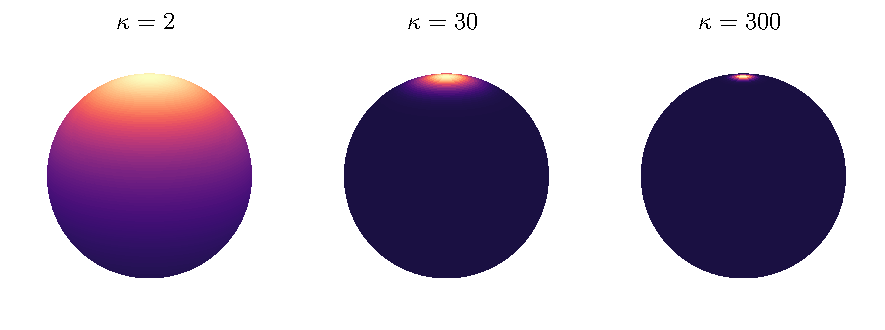
\includegraphics{figures/vmf_sphere.pdf}
    \caption{The von Mises--Fisher distribution on the sphere for three values of the concentration $\kappa$, with the mean direction $\boldsymbol\mu$ at the top. A small $\kappa$ spreads probability over a wide cap (an uncertain event). A large $\kappa$ concentrates it into a narrow one (a well-constrained event).}
    \label{fig:vmf_sphere}
\end{figure}

The model is otherwise the one from Section~\ref{sec:direction_reco}, the same DOM-token transformer with the same inputs and the same joint stopped and through-going training. The head now emits four numbers per event. Three are normalised into the mean direction $\boldsymbol\mu$, just as for $\hat{\mathbf{n}}$ in Section~\ref{sec:direction_reco}, and the fourth is mapped to a positive concentration $\kappa$. The opening-angle objective is replaced by the negative log-likelihood of the true direction $\mathbf{n}_{\mathrm{true}}$ under the predicted distribution,
\[
    \mathcal{L}_{\mathrm{vMF}}
    = -\log f_3(\mathbf{n}_{\mathrm{true}};\boldsymbol\mu,\kappa)
    = -\log\kappa + \log\sinh\kappa + \log(4\pi)
      - \kappa\,\boldsymbol\mu^\top\mathbf{n}_{\mathrm{true}}.
\]
The last term still rewards aligning $\boldsymbol\mu$ with the truth, so the point direction is learned for essentially the same reason as under the opening-angle loss. The new ingredient is that the same objective also forces $\kappa$ to be large only when that alignment is reliably good and small when it is not. The model is penalised both for being wrong and for being overconfident, and the $\kappa$ it settles on is a genuine learned per-event uncertainty rather than a nominal one.

Two practical points matter when training this head. First, $\sinh\kappa$ overflows for even moderately large $\kappa$, so the log-normalisation is evaluated through its asymptote $\log\sinh\kappa\to\kappa-\log 2$ rather than directly. Second, the likelihood rewards confidence without limit. For an event the model reconstructs well, the loss keeps decreasing as $\kappa$ grows, so left unchecked the network inflates $\kappa$ without bound to harvest ever more reward on the events it happens to get right. The training is therefore run more cautiously than for the point-estimate model, with a smaller learning rate, a small penalty on $\kappa$, and an upper bound on it.


Figure~\ref{fig:vmf_training} shows the resulting training history. Every event
receives a single $\kappa$, and the band shows the spread of these predictions
across the validation events, covering the central $80\%$ of them at each epoch,
between the 10th and 90th percentiles. The spread is wide, but the median settles
high, so the typical event is reconstructed with confidence.

\begin{figure}[H]
    \centering
    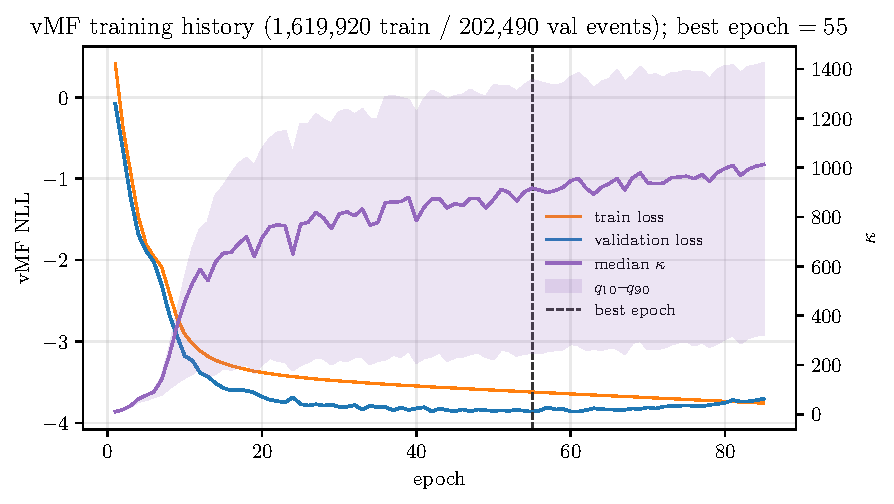
\includegraphics{figures/vmf_training_history_loss_opening_kappa.pdf}
    \caption{Training history of the vMF direction model. The weighted vMF
    negative log-likelihood for the training and validation sets is on the left
    axis. The median predicted concentration $\kappa$ with its 10th--90th
    percentile band is on the right. The dashed line marks the best validation epoch.}
    \label{fig:vmf_training}
\end{figure}

We now apply the trained model to both MC and data. Figure~\ref{fig:vmf_kappa} compares the
resulting $\kappa$ distributions for the two classes. The bulk of the two
distributions tracks closely in both cases.

\begin{figure}[H]
    \centering
    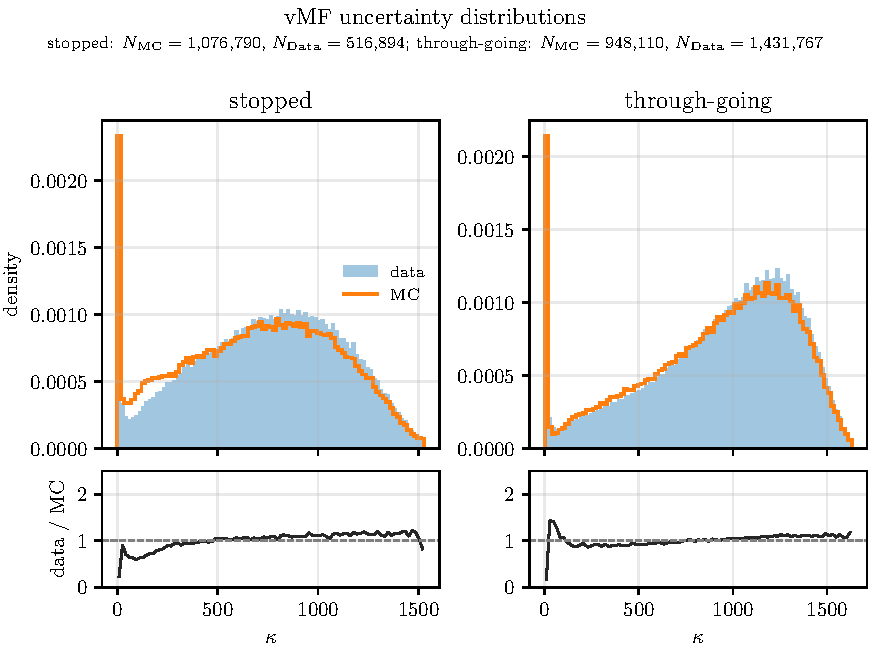
\includegraphics{figures/vmf_kappa_mc_data_stopped_through_side_by_side.pdf}
    \caption{Distributions of the predicted vMF concentration $\kappa$ for data
    and corrected MC, shown separately for stopped (left) and through-going
    (right) events. The bottom panels give the data/MC ratio.}
    \label{fig:vmf_kappa}
\end{figure}

The one clear disagreement sits at the lower edge of the range, where MC carries
a sharp spike of minimum-concentration events that the data does not match.
Figure~\ref{fig:vmf_pole_collapse} takes a closer look at these events. In the
left panel, where the MC truth is available, the predicted zenith of the MC
events with $\kappa<10$ piles up near the pole while their true zenith
distribution looks entirely different. The few data events with $\kappa<10$
show no such collapse, their predicted zenith instead following a broader,
if somewhat skewed, distribution. The right panel shows that the sharp MC spike
does not arise from low zenith angles as such, since the bulk of genuinely
vertical MC events receives a large $\kappa$. The $\kappa$ split in
Table~\ref{tab:kappa_split} suggests that the low $\kappa$ values in MC instead
arise from sparse observations. The MC events below the cut carry roughly half
the DOMs, pulses, and charge of the rest of the sample, so the collapse to low
zenith angles seems to be what the network falls back on when starved of
information, which the vMF head, to its credit, flags with a tiny $\kappa$.

\begin{figure}[H]
    \centering
    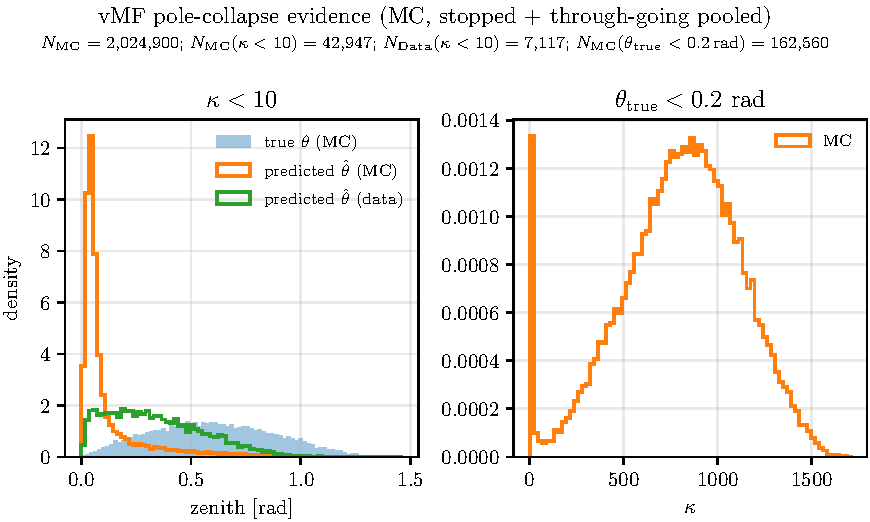
\includegraphics{figures/vmf_pole_collapse_evidence.pdf}
    \caption{Left, true and predicted zenith distributions for the MC events with
    $\kappa<10$, together with the predicted zenith of the data events with
    $\kappa<10$. Right, the $\kappa$ distribution for MC events with true zenith
    below $0.2\,\mathrm{rad}$. Stopped and through-going events are pooled in
    both panels.}
    \label{fig:vmf_pole_collapse}
\end{figure}

\begin{table}[H]
\centering
\small
\begin{tabular}{llcccc}
\toprule
Class & Selection & $N_{\mathrm{DOMs}}$ & $N_{\mathrm{pulses}}$ & $Q_{\mathrm{tot}}$ [PE] & $\kappa$ \\
\midrule
\multirow{2}{*}{stopped} & $\kappa < 10$ & 28 & 33 & 32 & 5.3 \\
                         & $\kappa \geq 10$    & 52 & 60 & 58 & 748 \\
\midrule
\multirow{2}{*}{through-going} & $\kappa < 10$ & 32 & 38 & 37 & 5.3 \\
                               & $\kappa \geq 10$    & 66 & 78 & 74 & 1011 \\
\bottomrule
\end{tabular}
\caption{Median event properties of the MC sample split at $\kappa=10$, shown
separately for stopped and through-going events.}
\label{tab:kappa_split}
\end{table}

This one-sided artefact is something a data--MC classifier could exploit, so we
remove the $\kappa<10$ events from both samples and retrain the MC-vs-data
transformer of Section~\ref{sec:data_mc_comparison} on what remains.

The test-set AUC falls to $0.9218$ for stopped events, from $0.9281$ after the
HLC re-labelling, and to $0.9848$ for through-going, from $0.9851$.


\chapter{Discussion and Conclusion}

This report set out to test whether simulated and real detector data look
sufficiently alike, the assumption on which essentially every downstream IceCube
machine-learning result depends on, and to repair as much of the disagreement as
possible. We did this by comparing two high-statistics samples of atmospheric muons, one
simulated with Monte Carlo and one drawn from the 2021 burnsample of real
detector data, where the muons were classified by a graph neural network
classifier~\cite{DenBestenPrivate}. Both are in the common
\texttt{SplitInIcePulses} data representation. The comparison was made with a
deliberately demanding yardstick. Rather than asking whether individual
distributions agree by eye, we trained a pulse-level transformer to separate
data from simulation and read off its test-set AUC. A value of $0.5$ would be consistent
with the two samples being statistically indistinguishable in our feature space, while
any excess above $0.5$ measures how much real and simulated muons can still be
told apart.

\section{Summary of the corrections}

The test itself was settled almost immediately. The benchmark classifier of
Section~\ref{subsec:single_metric} had no trouble telling the two samples apart,
so the assumption failed, and the work of the analysis shifted to the repair. Four corrections were afterwards applied in sequence, each
targeting its own discrepancy. The angular gradient-boosted reweighting
brought the reconstructed zenith and azimuth distributions of the MC muons into
agreement with data.
The pulse-merging step, adopted from Debes~\cite{simon}, folded a population of
sub-$0.3\,\mathrm{PE}$ HLC pulses into their above-threshold neighbours. Guided by a permutation-importance test
(Section~\ref{sec:feature_importance}, Table~\ref{tab:perm_importance_pulse})
that flagged the \texttt{hlc} flag as the single largest carrier of residual
data--MC distinguishability, we then re-labelled a class-dependent fraction of
the most HLC-like simulated SLC pulses, bringing the HLC-fraction distributions
into close agreement. Finally, a learned von Mises--Fisher concentration $\kappa$
exposed a population of low-information simulated events that the direction model
collapses toward the vertical. Removing these $\kappa<10$ events, from data and
MC alike so that the comparison stays fair, stripped out an artefact that the
benchmark classifier would otherwise exploit.

Table~\ref{tab:auc_summary} collects the resulting benchmark AUCs at each stage,
and Figure~\ref{fig:five_stage_logit_roc_overlay_combined} shows the
corresponding ROC curves.

\begin{table}[H]
\centering
\begin{tabular}{lcc}
\toprule
Stage & AUC (stopped) & AUC (through-going) \\
\midrule
Baseline (no correction)        & 0.9882 & 0.9960 \\
\;+\ angular GB reweighting       & 0.9688 & 0.9935 \\
\;+\ pulse merging                & 0.9583 & 0.9892 \\
\;+\ HLC re-labelling             & 0.9281 & 0.9851 \\
\;+\ removal of $\kappa<10$ events & 0.9218 & 0.9848 \\
\midrule
Total change                    & $-0.0664$ & $-0.0112$ \\
\bottomrule
\end{tabular}
\caption{Benchmark MC-vs-data test-set AUC of the pulse-level transformer at
each stage of the analysis, evaluated separately for stopped and through-going
muons. Each row adds one further correction on top of all previous ones.}
\label{tab:auc_summary}
\end{table}

\begin{figure}[H]
    \centering
    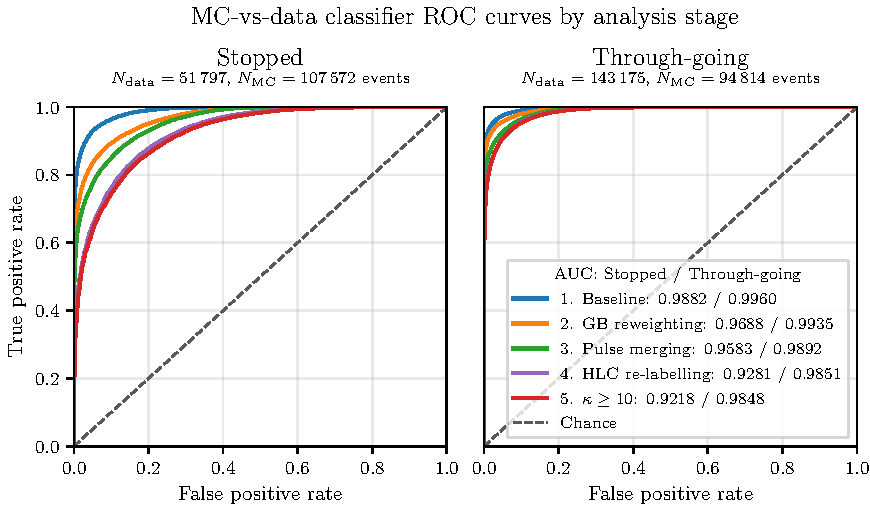
\includegraphics{figures/five_stage_logit_roc_overlay_combined.pdf}
    \caption{ROC curves of the MC-vs-data benchmark classifier at each stage of
    the analysis, for stopped (left) and through-going (right) events. The
    dashed diagonal marks the chance level.}
    \label{fig:five_stage_logit_roc_overlay_combined}
\end{figure}

The classifier starts out telling the two samples apart
more or less completely. Every correction then moves the benchmark in the right
direction, with the single largest step overall coming from the HLC
re-labelling, confirming that the permutation test had pointed at the most
consequential feature. Yet through all four corrections the AUC improves only modestly. For stopped
muons it falls from $0.9882$ to $0.9218$, for through-going muons barely at
all, from $0.9960$ to $0.9848$, and the ROC curves never come close to the
diagonal. Judged by rank alone, the two samples thus remain clearly separable,
especially the through-going ones. The unevenness also suggests that the
through-going events carry something the classifier exploits which the stopped
events do not carry, or at least not to the same degree. We never pursued this
systematically, but a direct stopped versus through-going comparison
would be a natural place for future work to start.



The logit distributions in Figure~\ref{fig:logit_catalog_common_xlim} show that
the corrections nevertheless changed more than the AUC lets on. The AUC is a
pure ranking statistic, asking only whether data events score above MC events,
not by how much. The logits show the margin. At baseline the classifier is
essentially certain about every event, with the two samples piled up in
well-separated peaks at large positive and negative logits. Correction by
correction the peaks contract toward zero and increasingly overlap, most
visibly at the HLC re-labelling and most dramatically for the stopped events,
where the once cleanly split distributions end up concentrated around the
decision boundary. It has become genuinely harder for the classifier to tell
the samples apart, even though it still can. It is safe to say that we have not
found every difference it can exploit, but we have thinned them out, and the
model is no longer nearly as confident in the separation.

Where the remaining separation sits is for future work to determine, but the
permutation test of Section~\ref{sec:feature_importance} offers a partial
guess. It ranked \texttt{dom\_time} second after the \texttt{hlc} flag, and
none of our corrections targets it directly.
Data showed a longer late-time tail there
(Figure~\ref{fig:pulse_level_variables_page1}). The afterpulses missing from
the simulation are a candidate explanation, although the search in
Section~\ref{sec:charge_time} could not confirm the connection. The horizontal coordinates
\texttt{dom\_x} and \texttt{dom\_y} also carried separation and were never
touched, since the angular reweighting mainly repaired the depth-like
variables. A mismatch here could well stem from data and MC muons not entering
the detector at the same points on the ice surface, a possibility this report has
not examined and a natural place for a future correction to start.

\begin{figure}[H]
    \centering
    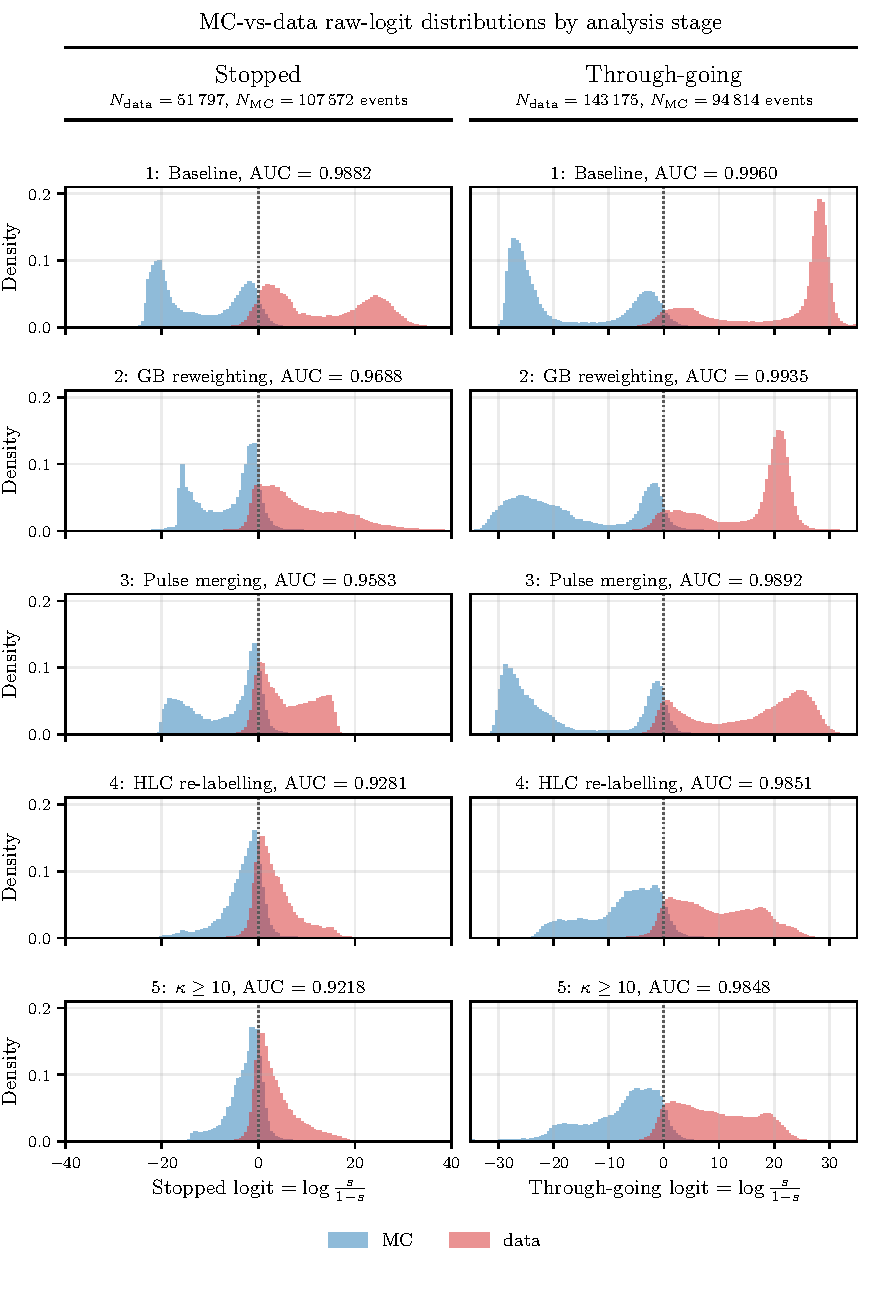
\includegraphics{figures/logit_catalog_common_xlim.pdf}
    \caption{Raw logit distributions of the MC-vs-data benchmark classifier at
    each stage of the analysis, for stopped (left) and through-going (right)
    events. The logit $\log\frac{s}{1-s}$ of the classifier score $s$ measures
    the per-event confidence, with the dotted line at zero marking indecision.}
    \label{fig:logit_catalog_common_xlim}
\end{figure}

\section{Worth looking into}

The summary above has already pointed out several places for future work to
start. A few more are worth adding. The afterpulse population could not be isolated in
the sample as a whole (Section~\ref{sec:charge_time}). That does not mean it is
absent. It may simply be too subtle to stand out in the pooled pulse-level
distributions of a low-energy muon sample, and a more targeted search, or a
sample at higher energies, may well succeed where ours did not.

The number of pulses per DOM was observed but never acted upon. Data records
more multi-pulse DOMs than MC, as seen in Figure~\ref{fig:pulses_per_dom}.

Most importantly, the muon classification of the real sample relies entirely on
the graph neural network classifier of den Besten~\cite{DenBestenPrivate}. The
whole analysis builds on it, and we never challenged it. If the classifier is
not perfect and neutrino events leak into the data sample, those events have no
counterpart in the pure-muon MC, and some of the residual separation could be
nothing more than this contamination. Validating the muon selection itself is
therefore well worth the effort. The same caution applies to our own
through-going/stopped classifier. The split was made at the very start of the
analysis by a model that had only ever seen MC, so the data events that differ
most from the simulation are precisely the ones it is least equipped to
classify, and they may have ended up in either class. Every per-class result in
this report rests on that split, so getting to the bottom of it might also help
explain the difference we see between through-going and stopped muons.

\section{Conclusion}

In conclusion, this report took a real and a simulated atmospheric-muon sample
that a classifier could separate almost perfectly and, through a sequence of
physically and mechanically motivated corrections, drove that separability down,
 most decisively through the data-driven re-labelling of HLC
pulses. Because IceCube machine-learning models are trained on simulation
before being applied to real data, any disagreement between the two is carried
into the results the models then produce on the real data. Our corrections made that
disagreement smaller, but they did not remove it. The final AUCs make that plain. We did not find everything,
and what remains unidentified is substantial enough to still give the
classifier a strong handle for telling the two samples apart. What the
corrections did strip away is the certainty. As the logit distributions of
Figure~\ref{fig:logit_catalog_common_xlim} showed, the separation that survives
rests on far smaller margins than the one we started from.
